%% LyX 2.4.1 created this file.  For more info, see https://www.lyx.org/.
%% Do not edit unless you really know what you are doing.
\documentclass[american]{article}
\usepackage[T1]{fontenc}
\usepackage[utf8]{inputenc}
\usepackage{geometry}
\geometry{verbose,tmargin=1cm,bmargin=1cm,lmargin=1cm,rmargin=1cm}
\usepackage{amsmath}
\usepackage{amssymb}
\usepackage{babel}
\usepackage{float}       % for [H] float placement
\usepackage{booktabs}    % for \toprule, \midrule, \bottomrule
\usepackage{natbib}      % for \citet, \citep
% Required for tikzpicture and drawing features
\usepackage{tikz}
\usetikzlibrary{shapes,arrows,calc}

\newtheorem{proposition}{Proposition}
\newtheorem{remark}{Remark}
\newtheorem{proof}{Proof}
\begin{document}

\section{Theoretical Interpretation}
\label{sec:theory}

The preceding experiments reveal a consistent pattern: ES and GRPO reach comparable task accuracy, yet ES accumulates weight changes two orders of magnitude larger, its update direction resembles a random direction on holdout tasks, and the two solutions are linearly connected with no loss barrier. We now develop a theoretical account that explains all of these phenomena within a unified framework.

\paragraph{Central claim: signal--diffusion decomposition}

On a landscape with low-rank task-relevant structure, the ES displacement decomposes into signal and noise along each eigendirection. Let $Q = \sum_k \lambda_k \mathbf{u}_k\mathbf{u}_k^\top$ be the landscape curvature and $\gamma_k := 1 - \frac{\alpha\sigma}{\sigma_R}\lambda_k$. Then (Appendix~\ref{appsec:solution_geometry}):
\begin{equation}\label{eq:es_decomposition}
    \theta_{\mathrm{ES}} - \theta_0
    = \sum_{k=1}^{d}\Big[
    \underbrace{(\gamma_k^T - 1)(\mathbf{u}_k^\top\theta_0)}_{\text{GD-like: } = 0 \text{ when } \lambda_k = 0}
    +\; \underbrace{\textstyle\sum_{t=1}^{T}\gamma_k^{t-1}\,(\mathbf{u}_k^\top\eta_{T-t})}_{\text{diffusion: present for all } k}
    \Big]\,\mathbf{u}_k,
\end{equation}
where $\eta_t \sim \mathcal{N}(0, \frac{\alpha^2}{N}I_d)$ is per-step isotropic noise. On task-relevant directions ($\lambda_k > 0$), $\gamma_k < 1$ and the signal term drives the iterate toward the optimum, just as gradient descent would (Proposition~\ref{prop:gd_displacement}). On flat directions ($\lambda_k = 0$), $\gamma_k = 1$, the signal vanishes, and the noise terms sum to a pure random walk. Since flat directions account for $d - r$ of $d$ dimensions with $r \ll d$, this diffusion dominates. Gradient descent, by contrast, has no noise term: $\theta_{\mathrm{GD}} - \theta_0$ lies entirely within the column space of $Q$ (Proposition~\ref{prop:gd_displacement}).

\paragraph{Why diffusion dominates}

On a flat landscape, the ES update is a pure random walk (proof in Appendix~\ref{appsec:flat_RW_scaling}):
$\Delta\theta_t \sim \mathcal{N}(0,\, \frac{\alpha^2}{N} I_d)$, so
$\mathbb{E}[\|\theta_T - \theta_0\|^{2}] = {\alpha^2 T d}/{N}$.
This scaling---linear in $T$ and $d$, inverse in $N$---persists as the off-manifold baseline even when the landscape has curvature. On linear and quadratic landscapes, we derive the full single-step statistics analytically (Propositions~\ref{prop:linear_landscape_step},~\ref{prop:quad_landscape_step}); in both cases the covariance is $\mathrm{Cov}[\Delta\theta] = \frac{\alpha^2}{N}I_d + \text{rank-}r\text{ task terms}$, so the isotropic component is unchanged. The on-manifold fraction of per-step squared displacement is (Appendix~\ref{appsec:linear_landscape_step}):
\begin{equation}\label{eq:rho}
    \rho
    = {(1 + (N{+}1)s)}\,/\,{(d + (N{+}1)s)},
\end{equation}
where $s := \sigma^{2}\|\mathbf{v}\|^{2}/\sigma_{R}^{2} \in [0,1]$ is the signal fraction. Since $N \ll d$ in practice ($N = 30$, $d \approx 4 \times 10^9$), $\rho$ is negligible. Over $T$ steps (Proposition~\ref{prop:es_displacement}):
\begin{equation}\label{eq:norm_hierarchy}
    \mathbb{E}\|\theta_{\mathrm{ES}} - \theta_0\|^2
    = \underbrace{\mathcal{O}(r)}_{\text{on-manifold}}
    + \underbrace{{\alpha^2 T(d{-}r)}/{N}}_{\text{off-manifold}}
    \approx {\alpha^2 T d}/{N}.
\end{equation}

\paragraph{Geometric consequences}

The decomposition yields a sharp hierarchy (Propositions~\ref{prop:gd_displacement}--\ref{prop:es_gd_difference}):
\begin{align}
    \|\theta_{\mathrm{GD}} - \theta_0\|^2 = \mathcal{O}(r), \qquad
    \mathbb{E}\|\theta_{\mathrm{ES}} - \theta_0\|^2 = \mathcal{O}(r) + \mathcal{O}(d), \qquad
    \mathbb{E}\|\theta_{\mathrm{ES}} - \theta_{\mathrm{GD}}\|^2 = \mathcal{O}(d), \label{eq:hierarchy}
\end{align}
and the expected cosine similarity scales as $\mathcal{O}(\sqrt{r/d})$ (Remark~\ref{rmk:cosine_similarity}): nearly orthogonal despite similar task performance. The key behavioral difference is on flat directions: GD freezes at initialization while ES diffuses with variance $\alpha^2 t/N$ (Propositions~\ref{prop:quad_landscape_dynamics},~\ref{prop:gd_quad_dynamics}).

\subsection{Empirical validation and explanatory power}

\textbf{Random walk scaling.}\;
For the full parameter vector, $\|\Delta\theta\|^2$ grows linearly with step count ($r = 0.9999$ for ES vs.\ $r = 0.875$ for GRPO; Figure~\ref{fig:weight_drift}). Inverting the slope yields $d_{\mathrm{eff}}/d_{\mathrm{total}} = 96.4\%$---nearly all dimensions behave as flat. Per-parameter analysis confirms this: 145 large weight matrices follow the scaling almost exactly ($d_{\mathrm{eff}}/d = 0.968 \pm 0.014$, $R^2 = 0.9999$), while normalization parameters deviate strongly ($d_{\mathrm{eff}}/d = 1.73 \pm 0.88$; Appendix~\ref{appsec:weight_drift_RW_stats}, Fig.~\ref{fig:d_ratio}). The $3.6\%$ deficit is interpretable as the task-relevant fraction where curvature constrains the walk.

\textbf{Explaining each observation.}\;
Eq.~\eqref{eq:es_decomposition} simultaneously accounts for:
\textit{Large update norms} (Table~\ref{tab:norms}): ES is dominated by the $\mathcal{O}(d)$ off-manifold term while GRPO stays at $\mathcal{O}(r)$, producing the ${\sim}100\times$ ratio.\;
\textit{Flat mode connectivity} (Fig.~\ref{fig:connectivity}): the $\theta_{\mathrm{ES}}$--$\theta_{\mathrm{GD}}$ line lies in the off-manifold subspace where loss is flat.\;
\textit{ES resembles random} (Fig.~\ref{fig:directional-perturbation}): off-manifold dominance dilutes directional curvature.\;
\textit{Holdout degradation} (Fig.~\ref{fig:holdout-perturbation}): the fine-tuning landscape sits atop a broad plateau of base-task performance; off-manifold perturbations beyond a certain radius degrade general capabilities regardless of task relevance, explaining the matched ES--random degradation profiles.

 \begin{figure}[!ht]
    \centering
    \includegraphics[width=0.88\linewidth]{Theory_Schematics/Schematics_Landscape.png}
    \caption{Schematic of the fine-tuning loss landscape. GRPO moves along the low-dimensional task-relevant subspace (red). ES accumulates both a task-relevant component and a large off-manifold random walk (blue), yielding a much larger displacement nearly orthogonal to GRPO. The two solutions are linearly connected because the off-manifold component is loss-invariant.}
    \label{fig:landscape_schematics}
\end{figure}

\begin{remark}
This behavior connects to a broader phenomenon: \citet{antognini2018pca_highdim_random_walk} showed that high-dimensional Ornstein--Uhlenbeck processes are dominated by their flattest dimensions. Similar random-walk-like drift has been observed in SGD-trained neural network weights and ES-optimized visual stimuli \citep{wang2022highperf_ES,wang2022tuninglandscape}, suggesting high degeneracy on flat subspaces is a generic feature of high-dimensional landscapes.
\end{remark}


% \appendix
\clearpage
\appendix

% \begin{proposition}[ES as Isotropic Random Walk on Flat Landscapes]
% On a flat reward landscape, the ES weight update $\Delta\theta$ follows an isotropic Gaussian distribution:
% \begin{equation}
% \Delta\theta \sim \mathcal{N}\!\left(0,\; \frac{\sigma^2}{4N}I_d\right)
% \end{equation}
% independent of the realized rewards $\{R_i\}$. Consequently, after $T$ steps the cumulative deviation satisfies:
% \begin{equation}
% \mathbb{E}\|\theta_T - \theta_0\|^2 = \frac{\sigma^2 T d}{4N}
% \end{equation}
% This exhibits diffusive scaling in both time $T$ and the parameter dimension $d$.
% \end{proposition}

% \begin{proposition}[Signal--Noise Decomposition on Linear Landscapes]
% On a linear reward landscape $R(\theta) = -\mathbf{v}^\top\theta$ with observation noise $\sigma_\xi$,
% the ES update decomposes into orthogonal signal and noise components:
% \begin{align}
% \mathbb{E}[P^{\parallel}\Delta\theta] &= -\frac{\sigma\alpha}{\sqrt{\sigma^2\|\mathbf{v}\|^2 + \sigma_\xi^2}}\,\mathbf{v}, 
% &\mathrm{Var}[P^{\parallel}\Delta\theta] &= \frac{\alpha^2(2\sigma^2\|\mathbf{v}\|^2+\sigma_\xi^2)}{N(\sigma^2\|\mathbf{v}\|^2+\sigma_\xi^2)}P^{\parallel}\nonumber \\
% \mathbb{E}[P^{\perp}\Delta\theta] &= 0, 
% &\mathrm{Var}[P^{\perp}\Delta\theta] &= \frac{\alpha^2}{N}P^{\perp}
% \end{align}
% The signal-to-noise ratio of the on-manifold update scales as:
% \begin{equation}
% \mathrm{SNR} = \sqrt{N}\cdot\frac{\sigma\|\mathbf{v}\|}{\sqrt{2\sigma^2\|\mathbf{v}\|^2 + \sigma_\xi^2}}
% \end{equation}
% In the noise-free limit $\sigma_\xi\to 0$, $\mathrm{SNR}\to\sqrt{N/2}$, revealing an irreducible floor
% set by the non-Gaussian ($\chi^2$) fluctuations of the on-manifold exploration. In the high-noise
% limit $\sigma_\xi \gg \sigma\|\mathbf{v}\|$, the SNR degrades as $\sqrt{N}\,\sigma\|\mathbf{v}\|/\sigma_\xi$,
% recovering the classical ES sample-complexity bound.
% \end{proposition}



% \begin{proposition}[ES as Isotropic Random Walk on Flat Landscapes]
% On a flat reward landscape, the ES weight update $\Delta\theta$ follows an isotropic Gaussian distribution:
% \begin{equation}
% \Delta\theta \sim \mathcal{N}\!\left(0,\; \frac{\sigma^2}{4N}I_d\right)
% \end{equation}
% independent of the realized rewards $\{R_i\}$. Consequently, after $T$ steps the cumulative deviation satisfies:
% \begin{equation}
% \mathbb{E}\|\theta_T - \theta_0\|^2 = \frac{\sigma^2 T d}{4N}
% \end{equation}
% This exhibits diffusive scaling in both time $T$ and the parameter dimension $d$.
% \end{proposition}

% \begin{proposition}[Signal--Noise Decomposition on Linear Landscapes]
% On a linear reward landscape $R(\theta) = -\mathbf{v}^\top\theta$ with observation noise $\sigma_\xi$,
% the ES update decomposes into orthogonal signal and noise components:
% \begin{align}
% \mathbb{E}[P^{\parallel}\Delta\theta] &= -\frac{\sigma\alpha}{\sqrt{\sigma^2\|\mathbf{v}\|^2 + \sigma_\xi^2}}\,\mathbf{v}, 
% &\mathrm{Var}[P^{\parallel}\Delta\theta] &= \frac{\alpha^2(2\sigma^2\|\mathbf{v}\|^2+\sigma_\xi^2)}{N(\sigma^2\|\mathbf{v}\|^2+\sigma_\xi^2)}P^{\parallel}\nonumber \\
% \mathbb{E}[P^{\perp}\Delta\theta] &= 0, 
% &\mathrm{Var}[P^{\perp}\Delta\theta] &= \frac{\alpha^2}{N}P^{\perp}
% \end{align}
% The signal-to-noise ratio of the on-manifold update scales as:
% \begin{equation}
% \mathrm{SNR} = \sqrt{N}\cdot\frac{\sigma\|\mathbf{v}\|}{\sqrt{2\sigma^2\|\mathbf{v}\|^2 + \sigma_\xi^2}}
% \end{equation}
% In the noise-free limit $\sigma_\xi\to 0$, $\mathrm{SNR}\to\sqrt{N/2}$, revealing an irreducible floor
% set by the non-Gaussian ($\chi^2$) fluctuations of the on-manifold exploration. In the high-noise
% limit $\sigma_\xi \gg \sigma\|\mathbf{v}\|$, the SNR degrades as $\sqrt{N}\,\sigma\|\mathbf{v}\|/\sigma_\xi$,
% recovering the classical ES sample-complexity bound.
% \end{proposition}



% \subsection{Theoretical results}

% \begin{proposition}[ES as Isotropic Random Walk on Flat Landscapes]
% On a flat reward landscape, the ES weight update $\Delta\theta$ follows an isotropic Gaussian distribution:
% \begin{equation}
% \Delta\theta \sim \mathcal{N}\!\left(0,\; \frac{\sigma^2}{4N}I_d\right)
% \end{equation}
% independent of the realized rewards $\{R_i\}$. Consequently, after $T$ steps the cumulative deviation satisfies:
% \begin{equation}
% \mathbb{E}\|\theta_T - \theta_0\|^2 = \frac{\sigma^2 T d}{4N}
% \end{equation}
% This exhibits diffusive scaling in both time $T$ and the parameter dimension $d$.
% \end{proposition}

% \begin{proposition}[Signal--Noise Decomposition on Linear Landscapes]
% On a linear reward landscape $R(\theta) = -\mathbf{v}^\top\theta$ with observation noise $\sigma_\xi$,
% the ES update decomposes into orthogonal signal and noise components:
% \begin{align}
% \mathbb{E}[P^{\parallel}\Delta\theta] &= -\frac{\sigma\alpha}{\sqrt{\sigma^2\|\mathbf{v}\|^2 + \sigma_\xi^2}}\,\mathbf{v}, 
% &\mathrm{Var}[P^{\parallel}\Delta\theta] &= \frac{\alpha^2(2\sigma^2\|\mathbf{v}\|^2+\sigma_\xi^2)}{N(\sigma^2\|\mathbf{v}\|^2+\sigma_\xi^2)}P^{\parallel}\nonumber \\
% \mathbb{E}[P^{\perp}\Delta\theta] &= 0, 
% &\mathrm{Var}[P^{\perp}\Delta\theta] &= \frac{\alpha^2}{N}P^{\perp}
% \end{align}
% The signal-to-noise ratio of the on-manifold update scales as:
% \begin{equation}
% \mathrm{SNR} = \sqrt{N}\cdot\frac{\sigma\|\mathbf{v}\|}{\sqrt{2\sigma^2\|\mathbf{v}\|^2 + \sigma_\xi^2}}
% \end{equation}
% In the noise-free limit $\sigma_\xi\to 0$, $\mathrm{SNR}\to\sqrt{N/2}$, revealing an irreducible floor
% set by the non-Gaussian ($\chi^2$) fluctuations of the on-manifold exploration. In the high-noise
% limit $\sigma_\xi \gg \sigma\|\mathbf{v}\|$, the SNR degrades as $\sqrt{N}\,\sigma\|\mathbf{v}\|/\sigma_\xi$,
% recovering the classical ES sample-complexity bound.
% \end{proposition}



% \begin{proposition}[ES as Isotropic Random Walk on Flat Landscapes]
% On a flat reward landscape, the ES weight update $\Delta\theta$ follows an isotropic Gaussian distribution:
% \begin{equation}
% \Delta\theta \sim \mathcal{N}\!\left(0,\; \frac{\sigma^2}{4N}I_d\right)
% \end{equation}
% independent of the realized rewards $\{R_i\}$. Consequently, after $T$ steps the cumulative deviation satisfies:
% \begin{equation}
% \mathbb{E}\|\theta_T - \theta_0\|^2 = \frac{\sigma^2 T d}{4N}
% \end{equation}
% This exhibits diffusive scaling in both time $T$ and the parameter dimension $d$.
% \end{proposition}

% \begin{proposition}[Signal--Noise Decomposition on Linear Landscapes]
% On a linear reward landscape $R(\theta) = -\mathbf{v}^\top\theta$ with observation noise $\sigma_\xi$,
% the ES update decomposes into orthogonal signal and noise components:
% \begin{align}
% \mathbb{E}[P^{\parallel}\Delta\theta] &= -\frac{\sigma\alpha}{\sqrt{\sigma^2\|\mathbf{v}\|^2 + \sigma_\xi^2}}\,\mathbf{v}, 
% &\mathrm{Var}[P^{\parallel}\Delta\theta] &= \frac{\alpha^2(2\sigma^2\|\mathbf{v}\|^2+\sigma_\xi^2)}{N(\sigma^2\|\mathbf{v}\|^2+\sigma_\xi^2)}P^{\parallel}\nonumber \\
% \mathbb{E}[P^{\perp}\Delta\theta] &= 0, 
% &\mathrm{Var}[P^{\perp}\Delta\theta] &= \frac{\alpha^2}{N}P^{\perp}
% \end{align}
% The signal-to-noise ratio of the on-manifold update scales as:
% \begin{equation}
% \mathrm{SNR} = \sqrt{N}\cdot\frac{\sigma\|\mathbf{v}\|}{\sqrt{2\sigma^2\|\mathbf{v}\|^2 + \sigma_\xi^2}}
% \end{equation}
% In the noise-free limit $\sigma_\xi\to 0$, $\mathrm{SNR}\to\sqrt{N/2}$, revealing an irreducible floor
% set by the non-Gaussian ($\chi^2$) fluctuations of the on-manifold exploration. In the high-noise
% limit $\sigma_\xi \gg \sigma\|\mathbf{v}\|$, the SNR degrades as $\sqrt{N}\,\sigma\|\mathbf{v}\|/\sigma_\xi$,
% recovering the classical ES sample-complexity bound.
% \end{proposition}



% \subsection{Theoretical results}
\subsection{Evolution Strategy on a Flat Landscape}
\label{prop:flat}
\begin{proposition}[Evolution Strategy on a Flat Landscape] 
\label{prop:flat_landscape_scaling}
  Let $R(\theta) = \text{const}$, so all reward variation arises from
  observation noise. Under the ES update
  $\Delta\theta = \frac{\alpha}{N}\sum_{i=1}^N Z_i \epsilon_i$
  with $\epsilon_i \sim \mathcal{N}(0, I_d)$ and z-scored rewards
  $Z_i$, the weight update is a pure isotropic random walk:
  \[
      \Delta\theta \sim \mathcal{N}\!\left(0,\, \frac{\alpha^2}{N} I_d\right),
      \qquad
      \mathbb{E}\bigl[\|\Delta\theta\|^2\bigr] = \frac{\alpha^2 d}{N}.
  \]
  After $T$ steps of ES with population size $N$, step size $\alpha$, and parameter dimension $d$, the cumulative deviation satisfies
  \[
      \mathbb{E}\bigl[\|\theta_T - \theta_0\|^2\bigr]
      = \frac{\alpha^2 T d}{N}
      = \frac{\sigma^2 T d}{4N},
  \]
  where the last equality substitutes $\alpha = \sigma/2$.
  In particular, the expected drift grows linearly in $T$ and $d$,
  and shrinks inversely in the batch size $N$. Proof in \ref{appsec:flat_RW_scaling}.
  \end{proposition}

  \subsection{Evolution Strategy on a Linear Landscape}
  \begin{proposition}[Evolution Strategy on a Linear Landscape] \label{prop:linear_landscape_step}
    Let $R(\theta) = -\mathbf{v}^\top\theta$ with observation noise
    $\sigma_\xi$. Define $\sigma_R^2 := \sigma^2\|\mathbf{v}\|^2 + \sigma_\xi^2$.
    The mean and covariance of the ES parameter update are 
    \begin{align}
        \mathbb{E}[\Delta\theta]
        &= \frac{-\alpha\sigma\,\mathbf{v}}{\sigma_R} \label{eq:es_linear_mean} \\
        \operatorname{Cov}[\Delta\theta]
        &= \frac{\alpha^2}{N}\,I_d
          + \frac{\alpha^2\sigma^2}{N\sigma_R^2}\,\mathbf{v}\mathbf{v}^\top \label{eq:es_linear_cov}
    \end{align}
    The mean update is purely aligned with the gradient direction $\mathbf{v}$,
    and the covariance consists of the same isotropic baseline as the flat landscape
    plus a rank-1 boost along $\mathbf{v}$.
    Relative to the quadratic case (Proposition~\ref{prop:quad_landscape_step}),
    the linear landscape produces identical expressions with $Q^2 = 0$:
    the curvature-dependent inflation of $\sigma_R^2$ and the anisotropic
    noise term $2\sigma^4 Q^2$ are both absent. Proof in \ref{appsec:linear_landscape_step}.
    \end{proposition}
    
    \begin{remark}[On-manifold alignment of ES update]
    \label{remark:2}
    Define the signal fraction
    $s := \sigma^2\|\mathbf{v}\|^2/\sigma_R^2 \in [0,1]$.
    The on-manifold fraction of total squared displacement is
    \[
        \rho :=
        \frac{\mathbb{E}\|P^{\parallel}\Delta\theta\|^2}
             {\mathbb{E}\|\Delta\theta\|^2}
        =
        \frac{1 + (N+1)\,s}
             {d + (N+1)\,s}.
    \]
    Hence: (i) without signal ($s=0$), $\rho = 1/d$, i.e.\ the update is
    purely diffusive; (ii) in the high-SNR limit ($s\to 1$), $\rho \to
    (N+2)/(d+N+1)$; (iii) $\rho$ increases monotonically in $s$ and $N$,
    and decreases in $d$. Since $N \ll d$ in practice, on-manifold movement
    per step is negligible relative to off-manifold diffusion.
    \end{remark}

  % \begin{proposition}[Evolution Strategy on a Linear Landscape] \label{prop:linear_landscape_step}
  % Let $R(\theta) = -\mathbf{v}^\top\theta$ with observation noise
  % $\sigma_\xi$. Define the signal-to-noise ratio
  % $s := \frac{\sigma^2\|\mathbf{v}\|^2}{\sigma^2\|\mathbf{v}\|^2 + \sigma_\xi^2} \in [0,1]$.
  % The on- and off-manifold components of the update decouple:
  % \[
  %     \mathbb{E}[P^{\parallel}\Delta\theta]
  %     = \frac{-\sigma\alpha\,\mathbf{v}}{\sqrt{\sigma^2\|\mathbf{v}\|^2+\sigma_\xi^2}},
  %     \qquad
  %     \mathbb{E}[P^{\perp}\Delta\theta] = 0,
  % \]
  % so the \emph{mean} update is purely aligned with the gradient direction
  % $\mathbf{v}$. The on-manifold fraction of total squared displacement is
  % \[
  %     \rho :=
  %     \frac{\mathbb{E}\|P^{\parallel}\Delta\theta\|^2}
  %          {\mathbb{E}\|\Delta\theta\|^2}
  %     =
  %     \frac{1 + (N+1)\,s}
  %          {d + (N+1)\,s}.
  % \]
  % Hence: (i) without signal ($s=0$), $\rho = 1/d$, i.e.\ the update is
  % purely diffusive; (ii) in the high-SNR limit ($s\to 1$), $\rho \to
  % (N+2)/(d+N+1)$; (iii) $\rho$ increases monotonically in $s$ and $N$,
  % and decreases in $d$. Since $N \ll d$ in practice, on-manifold movement
  % per step is negligible relative to off-manifold diffusion.
  % \end{proposition}
  
  \subsection{Evolution Strategy on a Quadratic Landscape}
  
  \begin{proposition}[Evolution Strategy on a Quadratic Landscape] \label{prop:quad_landscape_step}
  Let $R(\theta) = -\frac{1}{2}\theta^\top Q\theta$,  %with $Q \succeq 0$,
  current iterate $\theta_0$, and $\mathbf{v} := Q\theta_0$
  (the negative gradient). Define
  \[
      \sigma_R^2 := \sigma^2\|\mathbf{v}\|^2
                  + \tfrac{\sigma^4}{2}\operatorname{Tr}[Q^2]
                  + \sigma_\xi^2.
  \]
  The mean and covariance of the ES parameter update are
  \begin{align}
      \mathbb{E}[\Delta\theta]
      &= \frac{-\alpha\sigma\,\mathbf{v}}{\sigma_R}, \label{eq:es-quad-mean} \\
      \operatorname{Cov}[\Delta\theta]
      &= \frac{\alpha^2}{N\sigma_R^2}
        \left(
          \sigma^2\,\mathbf{v}\mathbf{v}^\top
          + 2\sigma^4 Q^2
          + \sigma_R^2\,I_d
        \right). \label{eq:es-quad-cov}
  \end{align}
  Relative to the linear case (Proposition~\ref{prop:linear_landscape_step}), the quadratic term $Q$ introduces two
  additional contributions: (i) a curvature-dependent inflation of
  $\sigma_R^2$ through $\operatorname{Tr}[Q^2]$, which \emph{attenuates}
  the mean gradient step; and (ii) an anisotropic noise term
  $2\sigma^4 Q^2/\sigma_R^2$ in the covariance, which increases
  update variance along the principal high curvature directions
  of $Q$. Proof in \ref{appsec:quad_landscape_step}.
  \end{proposition}
  
  \begin{remark}[On-manifold alignment on quadratic landscape]
    The on-manifold fraction of total expected squared displacement is
    \[
        \rho
        =
        \frac{(N+1)\,\sigma^2\|\mathbf{v}\|^2
              + 2\sigma^4\,\hat{\mathbf{v}}^\top Q^2\hat{\mathbf{v}}
              + \sigma_R^2}
             {(N+1)\,\sigma^2\|\mathbf{v}\|^2
              + 2\sigma^4\,\operatorname{Tr}[Q^2]
              + d\,\sigma_R^2},
    \]
    where $\hat{\mathbf{v}} := \mathbf{v}/\|\mathbf{v}\|$.
    Setting $Q^2 = 0$ and $\sigma_R^2 = \sigma^2\|\mathbf{v}\|^2 + \sigma_\xi^2$
    recovers the linear-landscape ratio $\rho = (1+(N{+}1)s)/(d+(N{+}1)s)$.
    The quadratic landscape modifies $\rho$ in two ways:
    the curvature inflates $\sigma_R^2$, which grows the isotropic term
    $d\,\sigma_R^2$ in the denominator;
    and the $2\sigma^4 Q^2$ noise splits between numerator
    (the projection $\hat{\mathbf{v}}^\top Q^2\hat{\mathbf{v}}$) and
    denominator (the full trace $\operatorname{Tr}[Q^2]$).
    When the gradient aligns with the high-curvature eigenvectors,
    much of the curvature-induced noise is on-manifold and $\rho$ is
    comparable to the linear case; when the curvature is predominantly
    orthogonal to $\hat{\mathbf{v}}$, the denominator grows while the
    numerator does not, suppressing $\rho$.
    \end{remark}

  \subsection{Dynamics of ES on Quadratic Landscape}
  
  \begin{proposition}[Dynamics of ES on Quadratic Landscape] \label{prop:quad_landscape_dynamics}
    Consider the simplified evolution
    \[
    \theta_{t+1} = H\theta_t + \eta_t, \qquad \eta_t \sim \mathcal{N}\!\left(0,\tfrac{\alpha^2}{N}I_d\right),
    \]
    where $H = I - \frac{\alpha\sigma}{\sigma_R}Q = \sum_k \left(1 - \frac{\alpha\sigma}{\sigma_R}\lambda_k\right)\mathbf{u}_k\mathbf{u}_k^\top$. 
    \footnote{$\sigma_R$ here is a fixed constant, not changing across iterations as in the full ES update in Equation \ref{eq:es-quadratic-sigmaR}.}
    Let $\gamma_k := 1 - \frac{\alpha\sigma}{\sigma_R}\lambda_k$ denote the contraction factor along eigendirection $\mathbf{u}_k$. Then the projected mean and variance evolve as
    \[
    \mathbb{E}[\mathbf{u}_k^\top\theta_t] = \gamma_k^t\,\mathbf{u}_k^\top\theta_0,
    \]
    \[
    \mathrm{Var}[\mathbf{u}_k^\top\theta_t] = \frac{\alpha^2}{N}\cdot\begin{cases} \dfrac{1 - \gamma_k^{2t}}{1-\gamma_k^2}, & \gamma_k^2 \neq 1, \\[6pt] t, & \gamma_k^2 = 1. \end{cases}
    \]
    The process converges in mean and variance along direction $\mathbf{u}_k$ if and only if $|\gamma_k| < 1$, i.e.,
    \[
    0 < \lambda_k < \frac{2\sigma_R}{\alpha\sigma}.
    \]
    In this regime, the asymptotic variance is
    \[
    \lim_{t\to\infty}\mathrm{Var}[\mathbf{u}_k^\top\theta_t] = \frac{\alpha^2}{N}\cdot\frac{1}{1-\gamma_k^2},
    \]
    and the convergence timescale is $\tau_k = -\log 2\,/\log\gamma_k^2$. Proof in \ref{appsec:quad_landscape_dynamics}.
    \end{proposition}
    
    \begin{remark}[Stability conditions]
    The three failure modes each correspond to a violation of $|\gamma_k|<1$. Flat directions ($\lambda_k = 0$) satisfy $\gamma_k = 1$, so both the mean and variance grow as a pure random walk: the optimizer drifts diffusively and never localizes. Concave directions ($\lambda_k < 0$) give $\gamma_k > 1$, causing exponential divergence of both mean and variance --- the landscape actively repels the iterates. Overly sharp convex directions ($\lambda_k \geq 2\sigma_R/\alpha\sigma$) give $|\gamma_k| \geq 1$ for a different reason: the ES step overshoots, analogous to gradient descent with too large a learning rate. Note that because the ES learning rate is $\alpha = \sigma/2$, this threshold becomes $\lambda_k = 4\sigma_R/\sigma^2$.
    \end{remark}
    
    \begin{remark}[Optimal curvature]
    Within the stable regime, the convergence speed and asymptotic variance are jointly controlled by $\gamma_k^2$. Directions with $\lambda_k \approx \sigma_R/\alpha\sigma$ achieve $\gamma_k \approx 0$, which simultaneously minimizes the convergence timescale ($\tau_k \to 1$ iteration) and the asymptotic variance ($\approx \alpha^2/N$). Directions near the stability boundary $\lambda_k \to 0^+$ or $\lambda_k \to (2\sigma_R/\alpha\sigma)^-$ suffer slow convergence and inflated variance. Thus the landscape curvature relative to the ratio $\sigma_R/\alpha\sigma$ plays the role of an effective condition number for the ES dynamics.
    \end{remark}

    \begin{remark}[Role of noise scale]
    The asymptotic variance $\frac{\alpha^2}{N(1-\gamma_k^2)}$ reveals the expected tension between exploration and precision: increasing the population size $N$ suppresses variance linearly, while the landscape geometry (through $\gamma_k^2$) sets a floor on the minimum achievable uncertainty. In well-conditioned directions, $1 - \gamma_k^2 \approx 2\frac{\alpha\sigma}{\sigma_R}\lambda_k$, so the asymptotic variance scales as $\frac{\alpha\sigma_R}{2N\sigma\lambda_k}$, inversely proportional to both curvature and the signal-to-noise ratio $\sigma/\sigma_R$.
    \end{remark}
\subsection{Dynamics of GD on Quadratic Landscape}
  \begin{proposition}[Dynamics of GD on Quadratic Landscape] \label{prop:gd_quad_dynamics}
Let $R(\theta) = -\frac{1}{2}\theta^\top Q\theta$ with $Q \succeq 0$,
and let gradient descent with learning rate $\beta$ iterate as
$\theta_{t+1} = (I - \beta Q)\,\theta_t$.
Define $H_{\mathrm{GD}} := I - \beta Q$ and let
$\gamma_k^{\mathrm{GD}} := 1 - \beta\lambda_k$. The iterate is
\[
    \theta_t = H_{\mathrm{GD}}^t\,\theta_0
    = \sum_{k=1}^{d}(\gamma_k^{\mathrm{GD}})^t\,(\mathbf{u}_k^\top\theta_0)\,\mathbf{u}_k.
\]
Direction $\mathbf{u}_k$ converges if and only if $|\gamma_k^{\mathrm{GD}}| < 1$, i.e.,
$0 < \lambda_k < 2/\beta$.
In this regime the convergence timescale is
$\tau_k^{\mathrm{GD}} = -\log 2\,/\,\log(\gamma_k^{\mathrm{GD}})^2$,
and the residual error is exactly zero: $\lim_{t\to\infty}\mathbf{u}_k^\top\theta_t = 0$. Proof in \ref{appsec:gd_quad_landscape}.
\end{proposition}

\begin{remark}[Stability conditions for GD]
The three failure modes mirror those of the ES dynamics
(Proposition~\ref{prop:quad_landscape_dynamics}):
flat directions ($\lambda_k = 0$) give $\gamma_k^{\mathrm{GD}} = 1$, so the iterate
is frozen at $\mathbf{u}_k^\top\theta_0$ for all $t$ --- unlike ES, where the iterate
drifts diffusively.
Concave directions ($\lambda_k < 0$) give $\gamma_k^{\mathrm{GD}} > 1$, causing
exponential divergence.
Overly sharp convex directions ($\lambda_k \geq 2/\beta$) give
$|\gamma_k^{\mathrm{GD}}| \geq 1$, and the iterate overshoots with growing or
non-decaying oscillations.
\end{remark}

% \begin{remark}[Optimal curvature and condition number for GD]
% Within the stable regime, the optimal eigenvalue is $\lambda_k = 1/\beta$, achieving
% $\gamma_k^{\mathrm{GD}} = 0$ and convergence in a single iteration.
% The overall convergence rate is governed by the slowest stable direction.
% For small learning rate $\beta\lambda_k \ll 1$,
% $\tau_k^{\mathrm{GD}} \approx 1/(2\beta\lambda_k)$, inversely proportional to
% curvature. The condition number $\kappa := \lambda_{\max}/\lambda_{\min}$
% (over positive eigenvalues) controls the ratio of fastest to slowest timescales.
% \end{remark}

% \begin{remark}[Comparison of ES and GD dynamics] \label{rmk:es_gd_comparison}
% The ES iteration (Proposition~\ref{prop:quad_landscape_dynamics}) and GD iteration
% are structurally identical with the correspondence
% $\beta \leftrightarrow \alpha\sigma/\sigma_R$, up to the additive noise $\eta_t$
% in the ES case. The key differences are:
% \begin{enumerate}
% \item \textbf{Effective learning rate.}
%   The ES effective learning rate $\alpha\sigma/\sigma_R$ is self-normalized by the
%   reward standard deviation $\sigma_R$, providing automatic step-size adaptation
%   absent in vanilla GD with fixed $\beta$.
% \item \textbf{Stability threshold.}
%   GD diverges when $\lambda_k > 2/\beta$; ES diverges when
%   $\lambda_k > 2\sigma_R/(\alpha\sigma)$. The ES threshold is typically more
%   permissive since $\sigma_R \geq \sigma_\xi$ inflates the bound, though at the
%   cost of a smaller effective step size.
% \item \textbf{Asymptotic residual.}
%   GD converges exactly to $\theta^* = 0$ along stable directions. ES converges only
%   in distribution, with asymptotic variance $\alpha^2/[N(1-(\gamma_k^{\mathrm{ES}})^2)]$
%   per direction. On flat directions, GD stays frozen while ES diffuses with variance
%   $\alpha^2 t/N$.
% \end{enumerate}
% These are summarized by:
% \[
% \renewcommand{\arraystretch}{1.4}
% \begin{array}{lcc}
% \hline
%  & \textbf{Gradient Descent} & \textbf{Evolution Strategy} \\ \hline
% \text{Eff.\ learning rate} & \beta & \alpha\sigma/\sigma_R \\
% \text{Contraction factor } \gamma_k & 1 - \beta\lambda_k & 1 - \frac{\alpha\sigma}{\sigma_R}\lambda_k \\
% \text{Stability bound} & \lambda_k < 2/\beta & \lambda_k < 2\sigma_R/(\alpha\sigma) \\
% \text{Optimal curvature} & \lambda_k = 1/\beta & \lambda_k = \sigma_R/(\alpha\sigma) \\
% \text{Residual error (stable)} & 0 & \frac{\alpha^2}{N(1-\gamma_k^2)} \\
% \text{Flat direction ($\lambda_k=0$)} & \text{frozen} & \text{diffusion } \sim \frac{\alpha^2 t}{N} \\
% \hline
% \end{array}
% \]
% \end{remark}
\subsection{GD displacement is low-dimensional}
\begin{proposition}[GD displacement is low-dimensional] \label{prop:gd_displacement}
Starting from $\theta_0$ on a rank-$r$ quadratic landscape ($r \ll d$), the GD displacement
\[
    \theta_{\mathrm{GD}} - \theta_0
    = \sum_{k:\,\lambda_k > 0}\bigl[(1-\beta\lambda_k)^T - 1\bigr](\mathbf{u}_k^\top\theta_0)\,\mathbf{u}_k
\]
lies entirely within the $r$-dimensional column space of $Q$, with
$\|\theta_{\mathrm{GD}} - \theta_0\|^2 = \mathcal{O}(r)$.
\end{proposition}

\subsection{ES displacement decomposes into signal and diffusion}
\begin{proposition}[ES displacement decomposes into signal and diffusion] \label{prop:es_displacement}
The ES displacement from initialization decomposes as
\[
    \theta_{\mathrm{ES}} - \theta_0
    = \underbrace{(H_{\mathrm{ES}}^T - I)\theta_0}_{\text{signal (on-manifold)}}
    + \underbrace{\sum_{t=1}^{T}H_{\mathrm{ES}}^{t-1}\,\eta_{T-t}}_{\text{noise (all directions)}}.
\]
The signal term lies within the column space of $Q$, identical in structure to the
GD displacement with $\beta \leftrightarrow \alpha\sigma/\sigma_R$.
The noise term has support in all $d$ dimensions. For $r \ll d$ and large $T$,
\[
    \mathbb{E}\|\theta_{\mathrm{ES}} - \theta_0\|^2
    = \underbrace{\mathcal{O}(r)}_{\text{on-manifold}}
    + \underbrace{\frac{\alpha^2 T(d-r)}{N}}_{\text{off-manifold diffusion}}
    \approx \frac{\alpha^2 T d}{N}.
\]
\end{proposition}

\subsection{ES--GD difference is off-manifold}
\begin{proposition}[ES--GD difference is off-manifold] \label{prop:es_gd_difference}
When both methods have converged on the active directions
($(\gamma_k^{\mathrm{ES}})^T \approx (\gamma_k^{\mathrm{GD}})^T \approx 0$),
the expected squared difference between the two solutions is dominated by
off-manifold diffusion:
\[
    \mathbb{E}\|\theta_{\mathrm{ES}} - \theta_{\mathrm{GD}}\|^2
    \approx \frac{\alpha^2 T(d-r)}{N}
    = \mathcal{O}(d).
\]
\end{proposition}

\begin{remark}[Geometric summary] \label{rmk:geometric_summary}
The three pairwise squared distances satisfy the hierarchy (for $r \ll d$, large $T$):
\begin{align*}
    \|\theta_{\mathrm{GD}} - \theta_0\|^2 &= \mathcal{O}(r), \\
    \mathbb{E}\|\theta_{\mathrm{ES}} - \theta_0\|^2 &= \mathcal{O}(r) + \mathcal{O}(d), \\
    \mathbb{E}\|\theta_{\mathrm{ES}} - \theta_{\mathrm{GD}}\|^2 &= \mathcal{O}(d).
\end{align*}
The GD displacement is low-dimensional and task-aligned.
The ES displacement superposes a comparable on-manifold component with a much larger
isotropic off-manifold diffusion.
The ES--GD difference is dominated by the off-manifold term alone, since both methods
converge to the same optimum within the active subspace.
This accounts for the empirical observation that ES achieves similar task performance
to GD (shared on-manifold signal) while being far from it in parameter space
(off-manifold diffusion).
\end{remark}

\begin{remark}[Cosine similarity between displacements] \label{rmk:cosine_similarity}
Since $\theta_{\mathrm{GD}} - \theta_0$ lies within the column space of $Q$
and the ES noise is zero-mean, the expected inner product picks up only the
on-manifold signal of ES. For large $T$ with both converged on active directions,
the expected cosine similarity satisfies
\[
    \mathbb{E}\left[\cos\angle(\theta_{\mathrm{ES}} - \theta_0,\;
    \theta_{\mathrm{GD}} - \theta_0)\right]
    \sim \mathcal{O}\!\left(\sqrt{r/d}\right),
\]
which is small for $r \ll d$: the two displacement vectors are nearly orthogonal
despite leading to similar task performance.
\end{remark}
  
  \section{Detailed derivations of theoretical results}
  
  \subsection{Z-score ES Update Setup}
  We detail the ES update rule as implemented in LLM fine-tuning. The update at step $t$ is
  \begin{equation}
    \theta_{t+1} = \theta_{t} + \alpha \cdot \frac{1}{N} \sum_{i=1}^{N} Z_{i} \epsilon_{i}
  \end{equation}
  where each $\epsilon_{i} \sim \mathcal{N}(0, I_{d})$ is an independent Gaussian perturbation, and $Z_{i} = \frac{R_{i} - \mu_{R}}{\sigma_{R}}$ is the z-scored return for the $i$-th sample. Here, $R_{i}$ is the reward, with $\mu_{R}$ and $\sigma_{R}$ denoting the mean and standard deviation of the $R_{i}$ across the population.
  With slight abuse of notation we let $R(\theta_{t} + \sigma \epsilon_{i})$ be the true or expected reward at the perturbed location, and $R_i$ the observed reward with certain observation noise.
  The step size is set to $\alpha = \sigma/2$, and a population size of $N = 30$ is typical. Defining the update increment as
  \begin{equation}
    \Delta\theta = \alpha \cdot \frac{1}{N} \sum_{i=1}^{N} Z_{i} \epsilon_{i}
  \end{equation}
  the algorithm iterates as $\theta_{t+1} = \theta_{t} + \Delta\theta$.
  
  \subsection{Flat Landscape Analysis}\label{appsec:flat_RW_scaling}

  \begin{proof}[Proof of Proposition~\ref{prop:flat_landscape_scaling}]
  The key assumption is that $Z_{i}$ is independent of $\epsilon_{i}$,
  i.e., $Z_{i}\perp\epsilon_{i}$. Then, conditioned on a set of $Z_{i}$,
  \begin{equation}
    \mathrm{Var}\left[\Delta\theta \,\middle|\, Z_{i}\right] = \left( \frac{\alpha^{2}}{N^{2}}\sum_{i=1}^N Z_i^2 \right) I_d
  \end{equation}
  and the distribution is isotropic Gaussian:
  \begin{equation}
  \Delta\theta|Z_{i} \sim \mathcal{N}\left(0, \left(\frac{\alpha^{2}}{N^{2}}\sum_{i=1}^{N}Z_{i}^{2}\right)I_{d}\right)
  \end{equation}

  By definition,\footnote{Note that this constraint depends on the implementation of the z-score
  $Z_{i} = \frac{R_{i}-\mu_{R}}{\sigma_{R}}$. In our code, we compute
  the standard deviation as $\sigma_{R}^{2} = \frac{1}{N}\sum_{i=1}^{N}(R_{i}-\mu_{R})^{2}$.
  In the unbiased variance estimator (denominator $N-1$), the identity reads $\sum_{i=1}^{N}Z_{i}^{2} = N-1$.}
  \begin{align}
  \sum_{i=1}^{N}Z_{i}^{2}
  &= \sum_{i=1}^{N} \left(\frac{R_{i}-\mu_{R}}{\sigma_{R}}\right)^{2} \notag\\
  &= \frac{1}{\sigma_{R}^{2}}\sum_{i=1}^{N}(R_{i} - \mu_{R})^{2} \notag\\
  &= N\quad\text{(or $N-1$ with unbiased estimator)}
  \end{align}

  Therefore, in general the scaling is:
  \begin{align}
    \mathrm{Var}[\Delta\theta|Z_{i}] &= \frac{\alpha^2}{N^2} N\, I_d \notag \\
    &= \frac{\alpha^2}{N} I_d
  \end{align}
  Since this is independent of $Z_i$, it follows after marginalizing:
  \begin{equation}
    \Delta\theta \sim \mathcal{N} \left( 0, \frac{\alpha^2}{N} I_d \right)
  \end{equation}
  \begin{equation}
    \mathrm{Var}[\Delta\theta] = \frac{\alpha^2}{N} I_d
  \end{equation}

  On a flat loss, $\Delta\theta$ is independent between steps, so after $T$ steps,
  the combined weight change is
  \begin{equation}
    \bar{\Delta\theta}_T = \theta_T - \theta_0 = \sum_{t=1}^T \Delta\theta_t
  \end{equation}
  and the total variance is
  \begin{equation}
    \mathrm{Var}[\bar{\Delta\theta}_T] = \frac{\alpha^2 T}{N} I_d
  \end{equation}
  The expected squared norm of total deviation is
  \begin{equation}
    \mathbb{E}\|\bar{\Delta\theta}_T\|^2 = \frac{\alpha^2 T d}{N}
  \end{equation}
  Finally, substituting $\alpha = \frac{\sigma}{2}$ gives
  \begin{equation}
    \frac{\alpha^2}{N} = \frac{\sigma^2}{4N}
  \end{equation}
  and
  \begin{equation}
    \mathbb{E}\|\bar{\Delta\theta}_T\|^2 = \frac{\sigma^2 T d}{4N}
  \end{equation}
  \end{proof}

  \subsection{Linear Landscape Analysis}\label{appsec:linear_landscape_step}
  \begin{proof}[Proof of Proposition~\ref{prop:linear_landscape_step}]
  Consider a linear landscape with i.i.d.\ observational noise $\xi\sim\mathcal{N}(0,1)$,
  assumed independent of $\epsilon$, i.e., $\xi\perp\epsilon$.
  The linear reward is
  \begin{equation}
    R(\theta) = -\mathbf{v}^\top\theta
  \end{equation}
  and the observed reward for each sample is
  \begin{align}
    R_i &= R(\theta_0+\sigma\epsilon_i) + \sigma_\xi \xi_i \notag \\
        &= -\mathbf{v}^\top(\theta_0+\sigma \epsilon_i) + \sigma_\xi \xi_i \notag \\
        &\equiv -\sigma\,\mathbf{v}^\top\epsilon_i + \sigma_\xi \xi_i
  \end{align}
  
  Decompose the exploration as
  \begin{align}
    \epsilon_i = \epsilon_i^\perp + \epsilon_i^\parallel
  \end{align}
  where
  \begin{align}
    P^\perp &:= I - \frac{\mathbf{v}\mathbf{v}^\top}{\|\mathbf{v}\|^2} \\
    P^\parallel &:= \frac{\mathbf{v}\mathbf{v}^\top}{\|\mathbf{v}\|^2}
  \end{align}
  so that
  $\epsilon_i^\perp := P^\perp \epsilon_i$, $\epsilon_i^\parallel := P^\parallel \epsilon_i$.
  Then $\epsilon_i^\perp \sim \mathcal{N}(0, P^\perp)$, $\epsilon_i^\parallel \sim \mathcal{N}(0, P^\parallel)$,
  and $\epsilon_i^\perp\perp\epsilon_i^\parallel$.

  The reward is
  \begin{align}
    R_i &= -\sigma \mathbf{v}^\top \epsilon_i^\parallel + \sigma_\xi \xi_i
  \end{align}
  and thus $R_i \perp \epsilon_i^\perp$.

  The update is:
  \begin{equation}
    \Delta\theta = \alpha \cdot \frac{1}{N} \sum_{i=1}^N Z_i \epsilon_i
  \end{equation}
  and can be split as
  \begin{equation}
    \Delta\theta = P^\perp \Delta\theta + P^\parallel \Delta\theta
  \end{equation}

  \paragraph{Off-manifold component}
  \begin{align}
    P^\perp \Delta\theta &= \alpha \cdot \frac{1}{N} \sum_{i=1}^N Z_i P^\perp \epsilon_i \notag \\
    &= \alpha \cdot \frac{1}{N} \sum_{i=1}^N Z_i \epsilon_i^\perp
  \end{align}
  
  Conditioned on the observed normalized reward $Z_{i}$, $P^{\perp}\Delta\theta$
  is a weighted sum of Gaussian random vectors, thus Gaussian:
  \begin{equation}
    P^\perp\Delta\theta \mid \{Z_i\}_{i=1}^N \sim \mathcal{N}\left(
      0, \frac{\alpha^2}{N^2} \sum_{i=1}^N Z_i^2 P^\perp
    \right)
  \end{equation}
  
  Since $\{Z_{i}\}_{i=1}^{N}$ are z-scored $\{R_{i}\}_{i=1}^{N}$, the sum satisfies the following identity.%
  \begin{equation}
    P^\perp\Delta\theta \mid \{Z_i\}_{i=1}^N \sim \mathcal{N}\left(
      0, \frac{\alpha^2}{N} P^\perp
    \right)
  \end{equation}
  
  Because of the following equations:
  \begin{align}
  \sigma_{R}^{2} &= \frac{1}{N}\sum_{i=1}^{N}(R_{i}-\mu_{R})^{2}\\
  Z_{i} &= \frac{R_{i}-\mu_{R}}{\sigma_{R}}
  \end{align}
  
  Thus, the conditional distribution is
  \begin{equation}
  P^{\perp}\Delta\theta\,\big|\;\{Z_{i}\}_{i=1}^{N} \sim \mathcal{N}\left(0, \frac{\alpha^{2}}{N^{2}} N P^{\perp}\right)
  \end{equation}
  
  Since the conditional distribution $P^{\perp}\Delta\theta\,\big|\;\{Z_{i}\}_{i=1}^{N}$
  is independent of the observed reward, marginalizing over $Z_{i}$ we have
  \begin{equation}
  P^{\perp}\Delta\theta \sim \mathcal{N}\left(0,\frac{\alpha^{2}}{N}P^{\perp}\right)
  \end{equation}
  
  The norm of the off-manifold component is
  \begin{align}
    \mathbb{E}\|P^\perp\Delta\theta\|^2 &= \mathrm{Tr}\left[ \frac{\alpha^2}{N} P^\perp \right] \notag \\
    &= \frac{\alpha^2}{N} (d-1)
  \end{align}

  \paragraph{On-manifold component}
  
  \begin{align}
  P^{\parallel}\Delta\theta &= \alpha\cdot\frac{1}{N}\sum_{i=1}^{N}Z_{i}P^{\parallel}\epsilon_{i} \notag\\
  &= \alpha\cdot\frac{1}{N}\sum_{i=1}^{N}Z_{i}\epsilon_{i}^{\parallel}
  \end{align}
  
  The on-manifold variable can be expressed as $\epsilon_{i}^{\parallel} = \frac{\mathbf{v}}{\|\mathbf{v}\|} n_{i}$,
  with $n_{i} \sim \mathcal{N}(0,1)$, thus the reward can be written as 
  \begin{align}
  R_{i} &= -\sigma\mathbf{v}^{\top} \epsilon_{i}^{\parallel} + \sigma_{\xi}\xi_{i} \notag\\
  &= -\sigma \frac{\mathbf{v}^{\top}\mathbf{v}}{\|\mathbf{v}\|} n_{i} + \sigma_{\xi}\xi_{i} \notag\\
  &= -\sigma\|\mathbf{v}\| n_{i} + \sigma_{\xi}\xi_{i}
  \end{align}
  
  Recall the definition of observed reward and z-score, 
  \begin{equation}
  Z_{i} = \frac{R_{i} - \mu_{R}}{\sigma_{R}}
  \end{equation}
  
  To simplify derivation, we use the population expectation and standard
  deviation here: 
  \begin{align}
  \mu_{R} &\approx \mathbb{E}[R_{i}] = 0\\
  \sigma_{R}^{2} &\approx \mathrm{Var}[R_{i}] = \sigma^{2}\|\mathbf{v}\|^{2} + \sigma_{\xi}^{2}
  \end{align}
  
  Under these simplifications,
  \begin{align}
  P^{\parallel}\Delta\theta &= \frac{\alpha}{N} \sum_{i=1}^{N} Z_{i} \epsilon_{i}^{\parallel} \notag\\
  &= \frac{\alpha}{N} \sum_{i=1}^{N} \frac{-\sigma\|\mathbf{v}\| n_{i} + \sigma_{\xi}\xi_{i} - \mu_{R}}{\sigma_{R}} n_{i} \frac{\mathbf{v}}{\|\mathbf{v}\|} \notag\\
  &= \frac{\alpha}{N\sigma_{R}}\sum_{i=1}^{N} (-\sigma\|\mathbf{v}\| n_{i} + \sigma_{\xi}\xi_{i}) n_{i} \frac{\mathbf{v}}{\|\mathbf{v}\|}
  \end{align}
  
  The expectation reads
  \begin{align}
  \mathbb{E}[P^{\parallel}\Delta\theta] =&~ \frac{\alpha}{N\sigma_{R}}\sum_{i=1}^{N} \mathbb{E}\left[ (-\sigma\|\mathbf{v}\| n_{i} + \sigma_{\xi}\xi_{i}) n_{i} \right] \frac{\mathbf{v}}{\|\mathbf{v}\|} \notag\\
  =&~\frac{\alpha}{N\sigma_{R}}\mathbb{E}[ -\sigma\|\mathbf{v}\| \sum_{i=1}^{N} n_{i}^{2} + \sigma_{\xi} \sum_{i=1}^{N}\xi_{i} n_{i} ]\frac{\mathbf{v}}{\|\mathbf{v}\|} \notag\\
  =&~\frac{\alpha}{N\sigma_{R}}(-\sigma\|\mathbf{v}\|N)\frac{\mathbf{v}}{\|\mathbf{v}\|} \notag\\
  =&~\frac{-\sigma\alpha}{\sigma_{R}}\mathbf{v} \notag\\
  =&~\frac{-\sigma\alpha\mathbf{v}}{\sqrt{\sigma^{2}\|\mathbf{v}\|^{2} + \sigma_{\xi}^{2}}}
  \end{align}
  where we used independence, $\mathbb{E}[\xi_{i} n_{i}]=0$, and $\mathbb{E}[\sum_{i=1}^{N} n_{i}^{2}] = N$. 
  
  Next, consider the variance. Consider the individual term, $X_{i} = -\sigma\|\mathbf{v}\| n_{i}^{2} + \sigma_{\xi}\xi_{i} n_{i}$,
  and its variance:
  \begin{align}
  \mathrm{Var}[X_{i}] =&~\mathbb{E}[(-\sigma\|\mathbf{v}\| n_{i}^{2} + \sigma_{\xi}\xi_{i} n_{i})^{2}]
  - \mathbb{E}[-\sigma\|\mathbf{v}\| n_{i}^{2} + \sigma_{\xi} \xi_{i} n_{i}]^{2} \notag\\
  =&~\mathbb{E}[ \sigma^{2}\|\mathbf{v}\|^{2} \underbrace{n_{i}^{4}}_{3}
  - 2\sigma\|\mathbf{v}\|\sigma_{\xi} \underbrace{\xi_{i}}_{0} \underbrace{n_{i}^{3}}_{0}
  + \sigma_{\xi}^{2} \underbrace{\xi_{i}^{2}}_{1} \underbrace{n_{i}^{2}}_{1}
  ] - (\sigma\|\mathbf{v}\|)^{2} \notag\\
  =&~3\sigma^{2}\|\mathbf{v}\|^{2} + \sigma_{\xi}^{2} - (\sigma\|\mathbf{v}\|)^{2} \notag\\
  =&~2\sigma^{2}\|\mathbf{v}\|^{2} + \sigma_{\xi}^{2}
  \end{align}
  
  Therefore,
  \begin{align}
  \mathrm{Var}[P^{\parallel}\Delta\theta] &= \frac{\alpha^{2}}{N^{2}\sigma_{R}^{2}}N\,\mathrm{Var}[X_{i}] \frac{\mathbf{v}\mathbf{v}^{\top}}{\|\mathbf{v}\|^{2}}
  \notag\\
  &= \frac{ \alpha^{2} (2\sigma^{2}\|\mathbf{v}\|^{2} + \sigma_{\xi}^{2}) }{ N \sigma_{R}^{2} } P^{\parallel} \notag\\
  &= \frac{ \alpha^{2} (2\sigma^{2}\|\mathbf{v}\|^{2} + \sigma_{\xi}^{2}) }{ N (\sigma^{2}\|\mathbf{v}\|^{2} + \sigma_{\xi}^{2}) } P^{\parallel}
  \end{align}
  
  \begin{align}
  \mathbb{E}[\|P^{\parallel}\Delta\theta\|^{2}] =&~ \mathrm{Tr}\left[\mathrm{Var}[P^{\parallel}\Delta\theta]\right] + \mathbb{E}[P^{\parallel}\Delta\theta]^{\top} \mathbb{E}[P^{\parallel}\Delta\theta] \notag\\
  =&~\frac{ \alpha^{2} (2\sigma^{2}\|\mathbf{v}\|^{2} + \sigma_{\xi}^{2}) }{ N ( \sigma^{2}\|\mathbf{v}\|^{2} + \sigma_{\xi}^{2} ) } + \frac{ (\sigma\alpha)^{2} \|\mathbf{v}\|^{2} }{ \sigma^{2}\|\mathbf{v}\|^{2} + \sigma_{\xi}^{2} } \notag\\
  =&~\frac{\alpha^{2}}{N} + \left(1 + \frac{1}{N}\right) \frac{ \sigma^{2}\|\mathbf{v}\|^{2} \alpha^{2} }{ \sigma^{2}\|\mathbf{v}\|^{2} + \sigma_{\xi}^{2} }
  \end{align}

  \paragraph{Overall distribution of the update}
Since the off-manifold component $P^{\perp}\Delta\theta$ is independent of the rewards
and hence of $P^{\parallel}\Delta\theta$, we can combine the on- and off-manifold results
to obtain the full single-step statistics. Writing $\sigma_{R}^{2} := \sigma^{2}\|\mathbf{v}\|^{2}+\sigma_{\xi}^{2}$,
\begin{align}
  \mathbb{E}[\Delta\theta] &= \frac{-\sigma\alpha\,\mathbf{v}}{\sigma_{R}}, \\
  \mathrm{Cov}[\Delta\theta]
  &= \frac{\alpha^{2}}{N}\,I_{d}
     + \frac{\alpha^{2}\sigma^{2}}{N\sigma_{R}^{2}}\,\mathbf{v}\mathbf{v}^\top.
\end{align}
The covariance has the same isotropic baseline $\frac{\alpha^2}{N}I_d$ as the flat landscape,
plus a rank-1 boost along the gradient direction. 
% Equivalently, in the
% $\{P^{\parallel}, P^{\perp}\}$ decomposition the on-manifold variance exceeds the
% off-manifold variance by a factor
% $(2\sigma^{2}\|\mathbf{v}\|^{2}+\sigma_{\xi}^{2})/\sigma_{R}^{2} \in [1,2]$,
% an inflation due to the non-Gaussian ($\chi^{2}$) fluctuations of $n_i^2$
% that persists even in the noise-free limit $\sigma_\xi \to 0$.
The total expected squared norm is
\begin{align}
\mathbb{E}\|\Delta\theta\|^{2}
&= \frac{\sigma^{2}\alpha^{2}\|\mathbf{v}\|^{2}}{\sigma_{R}^{2}}
 + \frac{\alpha^{2}d}{N}
 + \frac{\alpha^{2}\sigma^{2}\|\mathbf{v}\|^{2}}{N\,\sigma_{R}^{2}}.
\end{align}

\end{proof}
  
  \paragraph{Manifold Alignment of Update}
  
  Consider the ratio of the on- and off-manifold movement:
  \begin{equation}
  \mathbb{E}\left[ \|P^{\parallel}\Delta\theta\|^{2} \right] = \frac{\alpha^{2}}{N} + \left( 1 + \frac{1}{N} \right) \frac{ \sigma^{2}\|\mathbf{v}\|^{2}\alpha^{2} }{ \sigma^{2}\|\mathbf{v}\|^{2} + \sigma_{\xi}^{2} }
  \end{equation}
  \begin{equation}
  \mathbb{E}\|P^{\perp}\Delta\theta\|^{2} = \frac{\alpha^{2}(d-1)}{N}
  \end{equation}
  
  The fraction of on-manifold squared deviation in the total deviation is:
  \begin{align}
  \frac{ \mathbb{E}\left[\|P^{\parallel}\Delta\theta\|^2\right] }{ \mathbb{E}\left[\|\Delta\theta\|^2\right] }
  &= \frac{ \mathbb{E}\left[\|P^{\parallel}\Delta\theta\|^{2}\right] }{ \mathbb{E}\left[\|P^{\parallel}\Delta\theta\|^{2}\right] + \mathbb{E}\|P^{\perp}\Delta\theta\|^{2} } \notag\\
  &= \frac{ \frac{\alpha^{2}}{N} + \left(1 + \frac{1}{N}\right) \frac{ \sigma^{2} \|\mathbf{v}\|^{2} \alpha^{2} }{ \sigma^{2} \|\mathbf{v}\|^{2} + \sigma_{\xi}^{2} } }
    { \frac{ \alpha^{2}(d-1)}{N} + \frac{\alpha^{2}}{N} + \left(1 + \frac{1}{N}\right) \frac{ \sigma^{2}\|\mathbf{v}\|^{2} \alpha^{2} }{ \sigma^{2}\|\mathbf{v}\|^{2} + \sigma_{\xi}^{2} } } \notag\\
  &= \frac{ \frac{1}{N} + \frac{N+1}{N} \frac{ \sigma^{2} \|\mathbf{v}\|^{2} }{ \sigma^{2} \|\mathbf{v}\|^{2} + \sigma_{\xi}^{2} } }
    { \frac{d}{N} + \frac{N+1}{N} \frac{ \sigma^{2} \|\mathbf{v}\|^{2} }{ \sigma^{2}\|\mathbf{v}\|^{2} + \sigma_{\xi}^{2} } } \notag\\
  &= \frac{ 1 + (N+1) \frac{ \sigma^{2}\|\mathbf{v}\|^{2} }{ \sigma^{2}\|\mathbf{v}\|^{2} + \sigma_{\xi}^{2} } }
           { d + (N+1)\frac{ \sigma^{2}\|\mathbf{v}\|^{2} }{ \sigma^{2}\|\mathbf{v}\|^{2} + \sigma_{\xi}^{2} } }
  \end{align}
  
  where $s:=\frac{\sigma^{2}\|\mathbf{v}\|^{2}}{\sigma^{2}\|\mathbf{v}\|^{2}+\sigma_{\xi}^{2}}$. 
  
  This formulation reveals the key scaling relation of on and off manifold
  movement 
  \begin{itemize}
  \item Signal to noise ratio $s:=\frac{\sigma^{2}\|\mathbf{v}\|^{2}}{\sigma^{2}\|\mathbf{v}\|^{2}+\sigma_{\xi}^{2}}$
  , which range from $s\in[0,1]$
  \begin{itemize}
  \item When no gradient exists, $\|\mathbf{v}\|^{2}=0$, then independent
  of number of sample $N$, $\rho=1/d$. i.e. the norm on one axis among
  $d$ axis is $1/d$.
  \item Similarly, when $\sigma_{\xi}^{2}\gg\sigma^{2}\|\mathbf{v}\|^{2}$
  i.e. the reward noise variance is much higher than the variation of
  signal under exploration range $\sigma$, then it's effectively no
  gradient and no guidance. 
  \item In the other extreme, when very little reward noise, $\sigma_{\xi}^{2}\ll\sigma^{2}\|\mathbf{v}\|^{2}$,
  $s\approx1$, then $\rho=\frac{N+2}{d+N+1}$. 
  \item Via differentiation, one can show, $\rho$ monotonically depends on
  signal to noise ratio $s$
  \end{itemize}
  \item Full dimension $d$. Increase the full space dim $d$ will monotonically
  decrease the on manifold fraction $\rho$. 
  \item Sample size per generation $N$. Increase the sample size $N$ will
  monotonically increase the on manifold fraction $\rho$. 
  \begin{itemize}
  \item Note this scaling is almost linear, so to get half of the variance
  on manifold, one need $(N+1)s\approx d$. In reality, $d\sim10^{9}$
  , which makes this impossible. 
  \item In most realistic regimes $N\ll d$, which makes this on manifold
  ratio per step nearly negligible. 
  \end{itemize}
  \end{itemize}
  
  \clearpage
  \subsection{Quadratic landscape analysis} \label{appsec:quad_landscape_step}
  \begin{proof}[Proof of Proposition~\ref{prop:quad_landscape_step}]
  Consider a quadratic potential centered, i.e. peaked at the origin $\theta^{*}=0$.
  \begin{equation}
  R(\theta)=-\frac{1}{2}\theta^{\top}Q\theta
  \end{equation}
  At current state $\theta_{0}$, the reward at perturbed locations
  with observation noise are, where $\xi_{i}\sim\mathcal{N}(0,1)$,
  $\epsilon_{i}\sim\mathcal{N}(0,I_{d})$
  \begin{align}
  R_{i} & =R(\theta_{0}+\sigma\epsilon_{i})+\sigma_{\xi}\xi_{i}\notag\\
   & =-\frac{1}{2}(\theta_{0}+\sigma\epsilon_{i})^{\top}Q(\theta_{0}+\sigma\epsilon_{i})+\sigma_{\xi}\xi_{i}\notag\\
   & =-\frac{1}{2}\theta_{0}^{\top}Q\theta_{0}-\sigma\,\theta_{0}^{\top}Q\epsilon_{i}-\frac{\sigma^{2}}{2}\epsilon_{i}^{\top}Q\epsilon_{i}+\sigma_{\xi}\xi_{i}
  \end{align}
  Expectation of reward reads, which is the population mean of reward
  samples 
  \begin{equation}
  \mathbb{E}[R_{i}]=-\frac{1}{2}\theta_{0}^{\top}Q\theta_{0}-\frac{\sigma^{2}}{2}\mathrm{Tr}Q
  \end{equation}
  
  Center the rewards with population mean, we define 
  \begin{equation}
  \tilde{R}_{i}:=R_{i}-\mathbb{E}[R_{i}]
  \end{equation}
  
  Centered reward has three terms, linear $A$, quadratic \textbf{$B$},
  and noise $C$ 
  \begin{equation}
  \tilde{R}_{i}=\underbrace{-\sigma\,\theta_{0}^{\top}Q\epsilon_{i}}_{\text{linear }A}\underbrace{-\frac{\sigma^{2}}{2}(\epsilon_{i}^{\top}Q\epsilon_{i}-\mathrm{Tr}Q)}_{\text{quad }B}+\underbrace{\sigma_{\xi}\xi_{i}}_{\text{scalar noise }C}
  \end{equation}
  
  One can abbreviate $\mathbf{v}:=Q^{\top}\theta_{0}$ as the negative
  gradient. 
  
  The weight update reads, 
  \begin{align}
  \Delta\theta & =\alpha\cdot\frac{1}{N}\sum_{i=1}^{N}Z_{i}\epsilon_{i}\notag\\
   & =\frac{\alpha}{N\sigma_{R}}\sum_{i=1}^{N}\tilde{R}_{i}\epsilon_{i}
  \end{align}
  
  Since perturbations $\tilde{R}_{i}\epsilon_{i}$ are i.i.d. sampled
  \begin{equation}
  \mathbb{E}[\Delta\theta]=\frac{\alpha}{\sigma_{R}}\mathbb{E}[\tilde{R}_{i}\epsilon_{i}]
  \end{equation}
  and 
  \begin{equation}
  \mathrm{Cov}[\Delta\theta]=\frac{\alpha^{2}}{N\sigma_{R}^{2}}\mathrm{Cov}[\tilde{R}_{i}\epsilon_{i}]
  \end{equation}
  
  One observe that both $\tilde{R}_{i}$ and $\tilde{R}_{i}\epsilon_{i}$
  are \textbf{polynomial functions of gaussian random variables} $\epsilon_{i}$
  and $\xi_{i}$ (up to 3rd order), thus we can compute \textbf{their
  moment of any order} via Wick-Isserlis theorem \citep{wick1950evaluation,isserlis1918formula},
  including mean and covariance of them.
  
  Here are the specific calculations:
  
  \paragraph{Reward variance}
  
  Note that all three terms $A,B,C$ are centered 
  \begin{align}
  \mathbb{E}[A] & =0\notag\\
  \mathbb{E}[B] & =0\notag\\
  \mathbb{E}[C] & =0
  \end{align}
  
  Further $A\perp C$, $B\perp C$ due to independence of noise, and
  \begin{equation}
  \mathbb{E}[AB]=0
  \end{equation}
  
  as it only has polynomial of $\epsilon_{i}$ of odd order 1 and 3,
  thus its expectation is 0. Thus, $A,B,C$ are not correlated with
  one another. Thus, 
  \begin{align}
  \mathrm{Var}[\tilde{R}_{i}] & =\mathbb{E}[\tilde{R}_{i}^{2}]\notag\\
   & =\mathbb{E}[A^{2}]+\mathbb{E}[B^{2}]+\mathbb{E}[C^{2}]
  \end{align}
  
  all cross terms vanish due to no correlation.
  \begin{align}
  \mathbb{E}[A^{2}] & =\mathbb{E}[(-\sigma\,\theta_{0}^{\top}Q\epsilon_{i})\cdot(-\sigma\,\theta_{0}^{\top}Q\epsilon_{i})]\notag\\
   & =\sigma^{2}\theta_{0}^{\top}QQ^{\top}\theta_{0}\notag\\
   & =\sigma^{2}\|\mathbf{v}\|^{2}
  \end{align}
  \begin{equation}
  \mathbb{E}[C^{2}]=\sigma_{\xi}^{2}
  \end{equation}
  \begin{align}
  \mathbb{E}[B^{2}] & =\mathbb{E}[(\frac{\sigma^{2}}{2}(\epsilon_{i}^{\top}Q\epsilon_{i}-\mathrm{Tr}Q))^{2}]\notag\\
   & =\frac{\sigma^{4}}{4}\mathbb{E}[\epsilon_{i}^{\top}Q\epsilon_{i}\cdot(\epsilon_{i}^{\top}Q\epsilon_{i}-\mathrm{Tr}Q)-\mathrm{Tr}Q\cdot(\epsilon_{i}^{\top}Q\epsilon_{i}-\mathrm{Tr}Q)]\notag\\
   & =\frac{\sigma^{4}}{4}\Big(\mathbb{E}[\epsilon_{i}^{\top}Q\epsilon_{i}\cdot\epsilon_{i}^{\top}Q\epsilon_{i}]-(\mathrm{Tr}Q)^{2}\Big)
  \end{align}
  
  The first quintic polynomial of $\epsilon_{i}$ can be tackled by
  Wick-Isserelis theorem. With slight mis-use of notation, here we let
  $\epsilon_{a}$ denote the $a$th element of $\epsilon_{i}$ vector.
  
  Then 
  \begin{equation}
  \mathbb{E}[\epsilon_{a}\epsilon_{b}\epsilon_{c}\epsilon_{d}]=I_{ab}I_{cd}+I_{ad}I_{bc}+I_{ac}I_{bd}
  \end{equation}
  
  thus 
  \begin{align}
  \mathbb{E}[\epsilon_{i}^{\top}Q\epsilon_{i}\cdot\epsilon_{i}^{\top}Q\epsilon_{i}] & =\mathbb{E}[\sum_{a,b,c,d}Q_{ab}Q_{cd}\epsilon_{a}\epsilon_{b}\epsilon_{c}\epsilon_{d}]\notag\\
   & =\sum_{a,b,c,d}Q_{ab}Q_{cd}\mathbb{E}[\epsilon_{a}\epsilon_{b}\epsilon_{c}\epsilon_{d}]\notag\\
   & =\sum_{a,b,c,d}Q_{ab}Q_{cd}(\delta_{ab}\delta_{cd}+\delta_{ac}\delta_{bd}+\delta_{ad}\delta_{bc})\notag\\
   & =\mathrm{Tr}Q\mathrm{Tr}Q+\mathrm{Tr}[Q^{\top}Q]+\mathrm{Tr}[QQ]
  \end{align}
  
  Thus 
  \begin{align}
  \mathbb{E}[B^{2}] & =\frac{\sigma^{4}}{4}\Big(\mathbb{E}[\epsilon_{i}^{\top}Q\epsilon_{i}\cdot\epsilon_{i}^{\top}Q\epsilon_{i}]-(\mathrm{Tr}Q)^{2}\Big)\notag\\
   & =\frac{\sigma^{4}}{4}\Big((\mathrm{Tr}Q)^{2}+2\mathrm{Tr}[Q^{2}]-(\mathrm{Tr}Q)^{2}\Big)\notag\\
   & =\frac{\sigma^{4}}{2}\mathrm{Tr}[Q^{2}]
  \end{align}
  
  In sum, the population variance of reward reads, 
  \begin{equation}
  \mathrm{Var}[\tilde{R}_{i}]=\sigma^{2}\|\mathbf{v}\|^{2}+\frac{\sigma^{4}}{2}\mathrm{Tr}[Q^{2}]+\sigma_{\xi}^{2}
  \end{equation}
  
  and the population standard deviation is 
  \begin{equation}
  \sigma_{R}=\sqrt{\sigma^{2}\|\mathbf{v}\|^{2}+\frac{\sigma^{4}}{2}\mathrm{Tr}[Q^{2}]+\sigma_{\xi}^{2}}
  \end{equation}
  
  
  \paragraph{Expectation of parameter update}
  
  Next let's examine expectation of parameter change, where the key
  is $\mathbb{E}[\tilde{R}_{i}\epsilon_{i}]$, decomposing into three
  terms
  \begin{equation}
  \mathbb{E}[\tilde{R}_{i}\epsilon_{i}]=\mathbb{E}[A\epsilon_{i}]+\mathbb{E}[B\epsilon_{i}]+\mathbb{E}[C\epsilon_{i}]
  \end{equation}
  
  Second term vanish due to the odd order of Gaussian variable, 
  \begin{equation}
  \mathbb{E}[B\epsilon_{i}]=0
  \end{equation}
  
  Third term vanish due to independence $\epsilon_{i}\perp\xi_{i}$
  \begin{equation}
  \mathbb{E}[C\epsilon_{i}]=0
  \end{equation}
  
  First term is easy to calculate 
  \begin{align}
  \mathbb{E}[A\epsilon_{i}] & =\mathbb{E}[(-\sigma\,\theta_{0}^{\top}Q\epsilon_{i})\epsilon_{i}]\notag\\
   & =-\sigma\mathbb{E}[\epsilon_{i}(\epsilon_{i}^{\top}\mathbf{v})]\notag\\
   & =-\sigma\mathbf{v}
  \end{align}
  
  So in sum, 
  \begin{equation}
  \mathbb{E}[\tilde{R}_{i}\epsilon_{i}]=-\sigma\mathbf{v}
  \end{equation}
  
  \begin{align}
  \mathbb{E}[\Delta\theta] & =\frac{\alpha}{\sigma_{R}}\mathbb{E}[\tilde{R}_{i}\epsilon_{i}]\notag\\
   & =\frac{-\alpha\sigma\mathbf{v}}{\sigma_{R}}\notag\\
   & =\frac{-\alpha\sigma\mathbf{v}}{\sqrt{\sigma^{2}\|\mathbf{v}\|^{2}+\frac{\sigma^{4}}{2}\mathrm{Tr}[Q^{2}]+\sigma_{\xi}^{2}}}
  \end{align}
  
  which is on expectation aligned with local gradient direction, but
  scaled by signal to noise ratio. 
  
  \paragraph{Variance of parameter update}
  
  Finally, let's examine variance of parameter change, where the key
  is $\mathrm{Cov}[\tilde{R}_{i}\epsilon_{i}]$,
  \begin{align}
  \mathrm{Cov}[\tilde{R}_{i}\epsilon_{i}] & =\mathbb{E}[\tilde{R}_{i}\epsilon_{i}(\tilde{R}_{i}\epsilon_{i})^{\top}]-\mathbb{E}[\tilde{R}_{i}\epsilon_{i}]\mathbb{E}[\tilde{R}_{i}\epsilon_{i}]^{\top}\notag\\
   & =\mathbb{E}[\tilde{R}_{i}^{2}\epsilon_{i}\epsilon_{i}^{\top}]-\sigma^{2}\mathbf{v}\mathbf{v}^{\top}
  \end{align}
  
  Tackling the first term, using the same logic (odd order and independence)
  to eliminate terms, 
  \begin{align}
  \mathbb{E}[\tilde{R}_{i}^{2}\epsilon_{i}\epsilon_{i}^{\top}] & =\mathbb{E}[(A+B+C)^{2}\epsilon_{i}\epsilon_{i}^{\top}]\notag\\
   & =\mathbb{E}[(A^{2}+B^{2}+C^{2}+2AB+2BC+2AC)\epsilon_{i}\epsilon_{i}^{\top}]\notag\\
   & =\mathbb{E}[(A^{2}+B^{2}+C^{2})\epsilon_{i}\epsilon_{i}^{\top}]
  \end{align}
  
  Tackle $C$ term. 
  \begin{align}
  \mathbb{E}[C^{2}\epsilon_{i}\epsilon_{i}^{\top}] & =\mathbb{E}[C^{2}]\mathbb{E}[\epsilon_{i}\epsilon_{i}^{\top}]\notag\\
   & =\sigma_{\xi}^{2}I_{d}
  \end{align}
  
  Tackle \textbf{$A$} term
  
  \begin{align}
  \mathbb{E}[A^{2}\epsilon_{i}\epsilon_{i}^{\top}] & =\mathbb{E}[(-\sigma\,\theta_{0}^{\top}Q\epsilon_{i})^{2}\epsilon_{i}\epsilon_{i}^{\top}]\notag\\
   & =\sigma^{2}\mathbb{E}[(\mathbf{v}^{\top}\epsilon_{i})^{2}\epsilon_{i}\epsilon_{i}^{\top}]
  \end{align}
  
  using the same Wick theorem trick we have each element 
  \begin{align}
  \mathbb{E}[(\mathbf{v}^{\top}\epsilon_{i})^{2}\epsilon_{i}\epsilon_{i}^{\top}]_{cd} & =\mathbb{E}[\sum_{a,b}\mathbf{v}_{a}\mathbf{v}_{b}\epsilon_{a}\epsilon_{b}\epsilon_{c}\epsilon_{d}]\notag\\
   & =\sum_{a,b}\mathbf{v}_{a}\mathbf{v}_{b}\mathbb{E}[\epsilon_{a}\epsilon_{b}\epsilon_{c}\epsilon_{d}]\notag\\
   & =\sum_{a,b}\mathbf{v}_{a}\mathbf{v}_{b}(\delta_{ab}\delta_{cd}+\delta_{ac}\delta_{bd}+\delta_{ad}\delta_{cb})\notag\\
   & =\|\mathbf{v}\|^{2}\delta_{cd}+\mathbf{v}_{c}\mathbf{v}_{d}+\mathbf{v}_{d}\mathbf{v}_{c}
  \end{align}
  
  Thus, 
  \begin{equation}
  \mathbb{E}[A^{2}\epsilon_{i}\epsilon_{i}^{\top}]=\sigma^{2}(\|\mathbf{v}\|^{2}I_{d}+2\mathbf{v}\mathbf{v}^{\top})
  \end{equation}
  
  Finally, tackle $B$ term 
  \begin{align}
  \mathbb{E}[B^{2}\epsilon_{i}\epsilon_{i}^{\top}] & =\mathbb{E}[(\frac{\sigma^{2}}{2}(\epsilon_{i}^{\top}Q\epsilon_{i}-\mathrm{Tr}Q))^{2}\epsilon_{i}\epsilon_{i}^{\top}]\notag\\
   & =\frac{\sigma^{4}}{4}\mathbb{E}[\Big((\epsilon_{i}^{\top}Q\epsilon_{i})^{2}-2\mathrm{Tr}Q\cdot\epsilon_{i}^{\top}Q\epsilon_{i}+(\mathrm{Tr}Q)^{2}\Big)\epsilon_{i}\epsilon_{i}^{\top}]
  \end{align}
  
  where we encounter 2nd, 4th and 6th order terms. 
  
  2nd order term
  \begin{equation}
  \mathbb{E}[(\mathrm{Tr}Q)^{2}\epsilon_{i}\epsilon_{i}^{\top}]=(\mathrm{Tr}Q)^{2}I_{d}
  \end{equation}
  
  4th order term 
  \begin{align}
  \mathbb{E}[\epsilon_{i}^{\top}Q\epsilon_{i}\cdot\epsilon_{i}\epsilon_{i}^{\top}]_{cd} & =\mathbb{E}[\sum_{a,b}Q_{ab}\epsilon_{a}\epsilon_{b}\epsilon_{c}\epsilon_{d}]\notag\\
   & =\sum_{a,b}Q_{ab}(\delta_{ab}\delta_{cd}+\delta_{ac}\delta_{bd}+\delta_{ad}\delta_{cb})\notag\\
   & =\mathrm{Tr}Q\cdot\delta_{cd}+Q_{cd}+Q_{dc}
  \end{align}
  
  Thus
  \begin{align}
  \mathbb{E}[\epsilon_{i}^{\top}Q\epsilon_{i}\cdot\epsilon_{i}\epsilon_{i}^{\top}] & =\mathrm{Tr}Q\cdot I_{d}+Q+Q^{\top}\notag\\
   & =\mathrm{Tr}Q\cdot I_{d}+2Q
  \end{align}
  
  6th order term
  \begin{equation}
  \mathbb{E}[\Big((\epsilon_{i}^{\top}Q\epsilon_{i})^{2}\Big)\epsilon_{i}\epsilon_{i}^{\top}]_{ef}=\mathbb{E}[\sum_{a,b,c,d}Q_{ab}Q_{cd}\epsilon_{a}\epsilon_{b}\epsilon_{c}\epsilon_{d}\epsilon_{e}\epsilon_{f}]
  \end{equation}
  
  Note this has $C_{6}^{2}=15$ pairings, with some diagrammatic reasoning,
  we can find topologically we have three types 
  \begin{align}
  \mathbb{E}[\Big((\epsilon_{i}^{\top}Q\epsilon_{i})^{2}\Big)\epsilon_{i}\epsilon_{i}^{\top}]_{ef} & =\mathbb{E}[\sum_{a,b,c,d}Q_{ab}Q_{cd}\epsilon_{a}\epsilon_{b}\epsilon_{c}\epsilon_{d}\epsilon_{e}\epsilon_{f}]\notag\\
   & =\sum_{a,b,c,d}Q_{ab}Q_{cd}\Big(\underbrace{\delta_{ab}\delta_{cd}\delta_{ef}}_{1\text{case}}+\underbrace{\delta_{ac}\delta_{bd}\delta_{ef}+...}_{2\text{case}}+\notag\\
   & \quad\quad\underbrace{\delta_{ae}\delta_{bf}\delta_{cd}+...}_{4\text{case}}+\underbrace{\delta_{ae}\delta_{cf}\delta_{bd}+...}_{8\text{case}}\Big)\notag\\
   & =((\mathrm{Tr}Q)^{2}+2\mathrm{Tr}Q^{2})\delta_{ef}+4\mathrm{Tr}Q\cdot Q_{ef}+8[Q^{2}]_{ef}
  \end{align}
  
  Thus 
  \begin{equation}
  \mathbb{E}[\Big((\epsilon_{i}^{\top}Q\epsilon_{i})^{2}\Big)\epsilon_{i}\epsilon_{i}^{\top}]=((\mathrm{Tr}Q)^{2}+2\mathrm{Tr}Q^{2})I_{d}+4\mathrm{Tr}Q\cdot Q+8Q^{2}
  \end{equation}
  
  
  \begin{figure}[h]
      \centering
      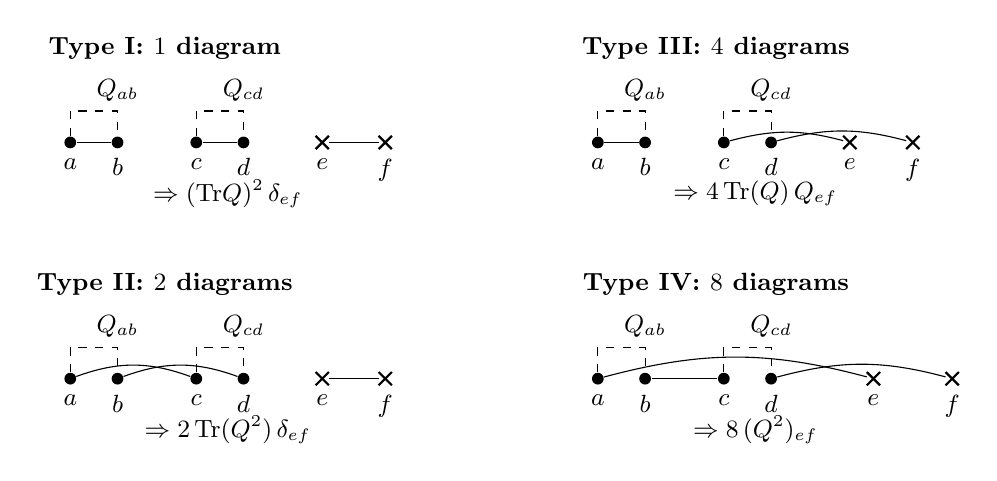
\begin{tikzpicture}[scale=1.0, every node/.style={font=\small}]
        % helper macro for Π-shaped Q edge
        \newcommand{\Qedge}[3]{
          \draw[dashed] (#1) |- ($(#1)!0.5!(#2)+(0,0.4)$) -| (#2)
            node[midway,above] {$#3$};
        }
      
        % helper macro for external cross node
        \newcommand{\crossnode}[3]{
          \node[draw, cross out, inner sep=2pt, line width=0.8pt, label=below:$#2$] (#1) at #3 {};
        }
      
        % -- Move titles up above diagrams to avoid overlap --
        % ---------- Type I ----------
        \node at (0,3.2) {\textbf{Type I: $1$ diagram}};
      
        \node[circle,fill=black,inner sep=1.5pt,label=below:$a$] (a1) at (-1.2,2) {};
        \node[circle,fill=black,inner sep=1.5pt,label=below:$b$] (b1) at (-0.6,2) {};
        \node[circle,fill=black,inner sep=1.5pt,label=below:$c$] (c1) at (0.4,2) {};
        \node[circle,fill=black,inner sep=1.5pt,label=below:$d$] (d1) at (1.0,2) {};
        \crossnode{e1}{e}{(2.0,2)}
        \crossnode{f1}{f}{(2.8,2)}
      
        \Qedge{a1}{b1}{Q_{ab}}
        \Qedge{c1}{d1}{Q_{cd}}
      
        \draw (e1) -- (f1);
        \draw (a1) to[out=0,in=180] (b1);
        \draw (c1) to[out=0,in=180] (d1);
      
        \node at (0.8,1.35) {$\Rightarrow (\mathrm{Tr}Q)^2\,\delta_{ef}$};
      
        % ---------- Type II ----------
        \node at (0,0.2) {\textbf{Type II: $2$ diagrams}};
      
        \node[circle,fill=black,inner sep=1.5pt,label=below:$a$] (a2) at (-1.2,-1) {};
        \node[circle,fill=black,inner sep=1.5pt,label=below:$b$] (b2) at (-0.6,-1) {};
        \node[circle,fill=black,inner sep=1.5pt,label=below:$c$] (c2) at (0.4,-1) {};
        \node[circle,fill=black,inner sep=1.5pt,label=below:$d$] (d2) at (1.0,-1) {};
        \crossnode{e2}{e}{(2.0,-1)}
        \crossnode{f2}{f}{(2.8,-1)}
      
        \Qedge{a2}{b2}{Q_{ab}}
        \Qedge{c2}{d2}{Q_{cd}}
      
        \draw (a2) to[out=20,in=160] (c2);
        \draw (b2) to[out=20,in=160] (d2);
        \draw (e2) -- (f2);
      
        \node at (0.8,-1.65) {$\Rightarrow 2\,\mathrm{Tr}(Q^2)\,\delta_{ef}$};
      
        % ---------- Type III ----------
        \node at (7,3.2) {\textbf{Type III: $4$ diagrams}};
      
        \node[circle,fill=black,inner sep=1.5pt,label=below:$a$] (a3) at (5.5,2) {};
        \node[circle,fill=black,inner sep=1.5pt,label=below:$b$] (b3) at (6.1,2) {};
        \node[circle,fill=black,inner sep=1.5pt,label=below:$c$] (c3) at (7.1,2) {};
        \node[circle,fill=black,inner sep=1.5pt,label=below:$d$] (d3) at (7.7,2) {};
        \crossnode{e3}{e}{(8.7,2)}
        \crossnode{f3}{f}{(9.5,2)}
      
        \Qedge{a3}{b3}{Q_{ab}}
        \Qedge{c3}{d3}{Q_{cd}}
      
        \draw (c3) to[out=15,in=165] (e3);
        \draw (d3) to[out=15,in=165] (f3);
        \draw (a3) to[out=0,in=180] (b3);
      
        \node at (7.5,1.35) {$\Rightarrow 4\,\mathrm{Tr}(Q)\,Q_{ef}$};
      
        % ---------- Type IV ----------
        \node at (7,0.2) {\textbf{Type IV: $8$ diagrams}};
      
          \node[circle,fill=black,inner sep=1.5pt,label=below:$a$] (a4) at (5.5,-1) {};
          \node[circle,fill=black,inner sep=1.5pt,label=below:$b$] (b4) at (6.1,-1) {};
          \node[circle,fill=black,inner sep=1.5pt,label=below:$c$] (c4) at (7.1,-1) {};
          \node[circle,fill=black,inner sep=1.5pt,label=below:$d$] (d4) at (7.7,-1) {};
          \crossnode{e4}{e}{(9.0,-1)}
          \crossnode{f4}{f}{(10.0,-1)}
  
          \Qedge{a4}{b4}{Q_{ab}}
          \Qedge{c4}{d4}{Q_{cd}}
  
          \draw (a4) to[out=15,in=165] (e4);
          \draw (b4) to[out=0,in=180] (c4);
          \draw (d4) to[out=15,in=165] (f4);
      
        \node at (7.5,-1.65) {$\Rightarrow 8\,(Q^2)_{ef}$};
      
      \end{tikzpicture}
      \caption{Wick contraction classes for $\mathbb{E}[(\epsilon^\top Q\epsilon)^2\,\epsilon_e\epsilon_f]$, with external loose ends $e,f$ shown as crosses.}
  \end{figure}
  
  
  In summary
  \begin{align}
  \mathbb{E}[B^{2}\epsilon_{i}\epsilon_{i}^{\top}] & =\frac{\sigma^{4}}{4}\mathbb{E}[\Big((\epsilon_{i}^{\top}Q\epsilon_{i})^{2}-2\mathrm{Tr}Q\cdot\epsilon_{i}^{\top}Q\epsilon_{i}+(\mathrm{Tr}Q)^{2}\Big)\epsilon_{i}\epsilon_{i}^{\top}]\notag\\
   & =\frac{\sigma^{4}}{4}\Big[((\mathrm{Tr}Q)^{2}+2\mathrm{Tr}Q^{2})I_{d}+4\mathrm{Tr}Q\cdot Q+8Q^{2}\notag\\
   & \quad-2\mathrm{Tr}Q\cdot(\mathrm{Tr}Q\cdot I_{d}+2Q)\notag\\
   & \quad+(\mathrm{Tr}Q)^{2}I_{d}\Big]\notag\\
   & =\frac{\sigma^{4}}{4}\Big[(2\mathrm{Tr}Q^{2})I_{d}+8Q^{2}\Big]\notag\\
   & =\frac{\sigma^{4}}{2}\Big[(\mathrm{Tr}Q^{2})\cdot I_{d}+4Q^{2}\Big]
  \end{align}
  
  Thus
  
  \begin{align}
  \mathbb{E}[\tilde{R}_{i}^{2}\epsilon_{i}\epsilon_{i}^{\top}] & =\mathbb{E}[(A^{2}+B^{2}+C^{2})\epsilon_{i}\epsilon_{i}^{\top}]\notag\\
   & =\sigma^{2}(\|\mathbf{v}\|^{2}I_{d}+2\mathbf{v}\mathbf{v}^{\top})+\frac{\sigma^{4}}{2}\Big[(\mathrm{Tr}Q^{2})\cdot I_{d}+4Q^{2}\Big]+\sigma_{\xi}^{2}I_{d}
  \end{align}
  
  The covariance term reads 
  \begin{align}
  \mathrm{Cov}[\tilde{R}_{i}\epsilon_{i}] & =\mathbb{E}[\tilde{R}_{i}^{2}\epsilon_{i}\epsilon_{i}^{\top}]-\sigma^{2}\mathbf{v}\mathbf{v}^{\top}\notag\\
   & =\sigma^{2}(\|\mathbf{v}\|^{2}I_{d}+\mathbf{v}\mathbf{v}^{\top})+\frac{\sigma^{4}}{2}\Big[(\mathrm{Tr}Q^{2})\cdot I_{d}+4Q^{2}\Big]+\sigma_{\xi}^{2}I_{d}
  \end{align}
  
  Recall that $\mathrm{Var}[\tilde{R}_{i}]=\sigma^{2}\|\mathbf{v}\|^{2}+\frac{\sigma^{4}}{2}\mathrm{Tr}[Q^{2}]+\sigma_{\xi}^{2}$
  
  \begin{equation}
  \mathrm{Cov}[\tilde{R}_{i}\epsilon_{i}]=\sigma^{2}\mathbf{v}\mathbf{v}^{\top}+2\sigma^{4}Q^{2}+\sigma_{R}^{2}I_{d}
  \end{equation}
  
  Thus in summary we have mean and covariance of parameter update, $\mathbf{v}:=Q\theta_{0}$
  \begin{align}
  \mathbb{E}[\Delta\theta] & =\frac{\alpha}{\sigma_{R}}\mathbb{E}[\tilde{R}_{i}\epsilon_{i}]\notag\\
   & =\frac{-\alpha\sigma\mathbf{v}}{\sigma_{R}}
  \end{align}
  \begin{align}
  \mathrm{Cov}[\Delta\theta] & =\frac{\alpha^{2}}{N\sigma_{R}^{2}}\mathrm{Cov}[\tilde{R}_{i}\epsilon_{i}]\notag\\
   & =\frac{\alpha^{2}}{N\sigma_{R}^{2}}\Big(\sigma^{2}\mathbf{v}\mathbf{v}^{\top}+2\sigma^{4}Q^{2}+\sigma_{R}^{2}I_{d}\Big)\notag\\
   & =\frac{\alpha^{2}}{N}I_{d}+\frac{\alpha^{2}}{N\sigma_{R}^{2}}\Big(\sigma^{2}\mathbf{v}\mathbf{v}^{\top}+2\sigma^{4}Q^{2}\Big)
  \end{align}
  
  The covariance of weight update has three terms 
  \begin{itemize}
  \item An isotropic variance term from the Gaussian exploration per se. $\frac{\alpha^{2}}{N}I_{d}$
  \item A rank-1 term along current gradient direction $\mathbf{v}$, $\frac{\alpha^{2}\sigma^{2}}{N\sigma_{R}^{2}}\mathbf{v}\mathbf{v}^{\top}$
  \item A term corresponding to landscape curvature, i.e. higher variance
  along higher curvature directions, $\frac{2\sigma^{4}\alpha^{2}}{N\sigma_{R}^{2}}Q^{2}$
  \end{itemize}
  \end{proof}
  
  \paragraph{Order analysis of quadratic landscape}

  Consider the relative magnitudes of the covariance terms, using the first term as a reference:
  \begin{itemize}
    \item The second term (aligned with the gradient direction) is of order $\frac{\sigma^{2}}{\sigma_{R}^{2}}\|\mathbf{v}\|^{2}$.
    \item The third term (along each direction $\mathbf{u}$) is of order $\frac{2\sigma^{4}}{\sigma_{R}^{2}}\,\mathbf{u}^{\top}Q^{2}\mathbf{u}$.
  \end{itemize}

  Since in practice $2\sigma^{2}$ is very small (e.g., $4.5\times10^{-6}$), the quadratic term generally acts as a small perturbation. To determine when the third (quadratic) term becomes comparable to the second, compare the terms along a specific direction $\mathbf{u}$:

  \begin{align}
    \frac{2\sigma^{4}}{\sigma_{R}^{2}}\,\mathbf{u}^{\top}Q^{2}\mathbf{u} &\approx \frac{\sigma^{2}}{\sigma_{R}^{2}}\|\mathbf{v}\|^{2} \notag\\
    2\sigma^{2}\,\mathbf{u}^{\top}Q^{2}\mathbf{u} &\approx \theta_{0}^{\top}Q^{2}\theta_{0} \notag\\
    \mathbf{u}^{\top}Q^{2}\mathbf{u} &\approx \frac{1}{2\sigma^{2}}\,\theta_{0}^{\top}Q^{2}\theta_{0}
  \end{align}

  
  Assume $\mathbf{u}$ is an eigenvector of $Q$ with eigenvalue $\lambda_{k}$,
  \begin{align}
  \lambda_{k}^{2} & \approx\frac{1}{2\sigma^{2}}\theta_{0}^{\top}Q^{2}\theta_{0}\notag\\
  \lambda_{k} & \approx\frac{\|\mathbf{v}\|}{\sqrt{2}\sigma}
  \end{align}
  \begin{equation}
  \lambda_{k}^{2}\approx\frac{1}{2\sigma^{2}}\sum_{i=1}^{d}\lambda_{i}^{2}(\theta_{0}^{\top}\mathbf{u}_{i})^{2}
  \end{equation}
  
  This shows that the current gradient norm $\|\mathbf{v}\|$ needs
  to be much smaller (at least $\sigma$ times) and the eigenvalue /
  curvature of the probe direction needs to be sharp enough for the
  3rd term to be comparable to the 2nd term. Two scenarios this could
  happen 
  \begin{itemize}
  \item For really sharply curved directions $\lambda_{k}$ this is usually
  be true. 
  \item The current state $\theta_{0}$ is close to optimum $\theta^{*}=0$
  or lies in the vast valley of degenerate solution, i.e. $Q\theta_{0}=0$,
  $\theta_{0}$ in the null space of $Q$. 
  \end{itemize}
  \paragraph{Manifold Alignment of Update}

Define the projections onto the gradient direction $\mathbf{v} = Q\theta_0$ and its orthogonal complement:
\begin{align}
P^{\parallel} &:= \frac{\mathbf{v}\mathbf{v}^{\top}}{\|\mathbf{v}\|^{2}}, \qquad
P^{\perp} := I_{d} - P^{\parallel}.
\end{align}

The on-manifold expected squared norm decomposes as
\begin{align}
\mathbb{E}\|P^{\parallel}\Delta\theta\|^{2}
&= \|\mathbb{E}[P^{\parallel}\Delta\theta]\|^{2}
   + \mathrm{Tr}[\mathrm{Cov}[P^{\parallel}\Delta\theta]].
\end{align}

For the first term, since $\mathbb{E}[\Delta\theta] = \frac{-\alpha\sigma\,\mathbf{v}}{\sigma_{R}}$
is already along $\mathbf{v}$, we have $P^{\parallel}\mathbb{E}[\Delta\theta] = \mathbb{E}[\Delta\theta]$, so
\begin{align}
\|\mathbb{E}[P^{\parallel}\Delta\theta]\|^{2}
&= \|\mathbb{E}[\Delta\theta]\|^{2}
= \frac{\alpha^{2}\sigma^{2}\|\mathbf{v}\|^{2}}{\sigma_{R}^{2}}.
\end{align}

For the second term, we project the covariance \eqref{eq:es-quad-cov} onto $P^{\parallel}$:
\begin{align}
\mathrm{Cov}[P^{\parallel}\Delta\theta]
&= P^{\parallel}\,\mathrm{Cov}[\Delta\theta]\,P^{\parallel} \notag\\
&= \frac{\alpha^{2}}{N\sigma_{R}^{2}}
   P^{\parallel}\left(\sigma^{2}\,\mathbf{v}\mathbf{v}^{\top}
   + 2\sigma^{4}Q^{2}
   + \sigma_{R}^{2}\,I_{d}\right)P^{\parallel}.
\end{align}
Evaluating each term using $P^{\parallel}\mathbf{v}\mathbf{v}^{\top}P^{\parallel} = \|\mathbf{v}\|^{2}P^{\parallel}$,
$P^{\parallel}Q^{2}P^{\parallel} = (\hat{\mathbf{v}}^{\top}Q^{2}\hat{\mathbf{v}})\,P^{\parallel}$
where $\hat{\mathbf{v}} := \mathbf{v}/\|\mathbf{v}\|$,
and $P^{\parallel}I_{d}\,P^{\parallel} = P^{\parallel}$:
\begin{align}
\mathrm{Cov}[P^{\parallel}\Delta\theta]
&= \frac{\alpha^{2}}{N\sigma_{R}^{2}}
   \left(\sigma^{2}\|\mathbf{v}\|^{2}
         + 2\sigma^{4}\,\hat{\mathbf{v}}^{\top}Q^{2}\hat{\mathbf{v}}
         + \sigma_{R}^{2}\right)P^{\parallel}.
\end{align}
Taking the trace ($\mathrm{Tr}[P^{\parallel}] = 1$) and combining:
\begin{align}
\mathbb{E}\|P^{\parallel}\Delta\theta\|^{2}
&= \frac{\alpha^{2}\sigma^{2}\|\mathbf{v}\|^{2}}{\sigma_{R}^{2}}
   + \frac{\alpha^{2}}{N\sigma_{R}^{2}}
     \left(\sigma^{2}\|\mathbf{v}\|^{2}
           + 2\sigma^{4}\,\hat{\mathbf{v}}^{\top}Q^{2}\hat{\mathbf{v}}
           + \sigma_{R}^{2}\right).
\end{align}

The total expected squared norm follows analogously using $\mathrm{Tr}[\mathbf{v}\mathbf{v}^{\top}] = \|\mathbf{v}\|^{2}$,
$\mathrm{Tr}[Q^{2}] = \mathrm{Tr}[Q^{2}]$, and $\mathrm{Tr}[I_{d}] = d$:
\begin{align}
\mathbb{E}\|\Delta\theta\|^{2}
&= \frac{\alpha^{2}\sigma^{2}\|\mathbf{v}\|^{2}}{\sigma_{R}^{2}}
   + \frac{\alpha^{2}}{N\sigma_{R}^{2}}
     \left(\sigma^{2}\|\mathbf{v}\|^{2}
           + 2\sigma^{4}\,\mathrm{Tr}[Q^{2}]
           + d\,\sigma_{R}^{2}\right).
\end{align}

Factoring out $\alpha^{2}/(N\sigma_{R}^{2})$ from both expressions --- noting that the
mean-squared term $\frac{\alpha^{2}\sigma^{2}\|\mathbf{v}\|^{2}}{\sigma_{R}^{2}}$
contributes $N\,\sigma^{2}\|\mathbf{v}\|^{2}$ after extracting the common factor,
which combines with the variance contribution to yield $(N+1)\,\sigma^{2}\|\mathbf{v}\|^{2}$
--- the on-manifold fraction is
\begin{align}
\rho
:= \frac{\mathbb{E}\|P^{\parallel}\Delta\theta\|^{2}}
        {\mathbb{E}\|\Delta\theta\|^{2}}
= \frac{(N+1)\,\sigma^{2}\|\mathbf{v}\|^{2}
        + 2\sigma^{4}\,\hat{\mathbf{v}}^{\top}Q^{2}\hat{\mathbf{v}}
        + \sigma_{R}^{2}}
       {(N+1)\,\sigma^{2}\|\mathbf{v}\|^{2}
        + 2\sigma^{4}\,\mathrm{Tr}[Q^{2}]
        + d\,\sigma_{R}^{2}}.
\end{align}

Setting $Q^{2}=0$ and $\sigma_{R}^{2}=\sigma^{2}\|\mathbf{v}\|^{2}+\sigma_{\xi}^{2}$
recovers the linear-landscape ratio $\rho = (1+(N+1)s)/(d+(N+1)s)$
with $s = \sigma^{2}\|\mathbf{v}\|^{2}/\sigma_{R}^{2}$.
  % \paragraph{Manifold Alignment of Update}

  % From equations above, the on-manifold expected squared norm is
  % \begin{align*}
  % \mathbb{E}\|P^{\parallel}\Delta\theta\|^{2}
  % &= \|\mathbb{E}[P^{\parallel}\Delta\theta]\|^{2}
  %    + \mathrm{Tr}[\mathrm{Cov}[P^{\parallel}\Delta\theta]] \\
  % &= \frac{\alpha^{2}\sigma^{2}\|\mathbf{v}\|^{2}}{\sigma_{R}^{2}}
  %    + \frac{\alpha^{2}}{N\sigma_{R}^{2}}
  %      \left(\sigma^{2}\|\mathbf{v}\|^{2}
  %            + 2\sigma^{4}\,\hat{\mathbf{v}}^{\top}Q^{2}\hat{\mathbf{v}}
  %            + \sigma_{R}^{2}\right)
  % \end{align*}
  % where $\hat{\mathbf{v}} := \mathbf{v}/\|\mathbf{v}\|$, using
  % $\mathrm{Tr}[\mathbf{v}\mathbf{v}^{\top}P^{\parallel}] = \|\mathbf{v}\|^{2}$,
  % $\mathrm{Tr}[Q^{2}P^{\parallel}] = \hat{\mathbf{v}}^{\top}Q^{2}\hat{\mathbf{v}}$,
  % and $\mathrm{Tr}[P^{\parallel}] = 1$.
  
  % Similarly, the total expected squared norm is
  % \begin{align*}
  % \mathbb{E}\|\Delta\theta\|^{2}
  % &= \frac{\alpha^{2}\sigma^{2}\|\mathbf{v}\|^{2}}{\sigma_{R}^{2}}
  %    + \frac{\alpha^{2}}{N\sigma_{R}^{2}}
  %      \left(\sigma^{2}\|\mathbf{v}\|^{2}
  %            + 2\sigma^{4}\,\mathrm{Tr}[Q^{2}]
  %            + d\,\sigma_{R}^{2}\right)
  % \end{align*}
  % using $\mathrm{Tr}[\mathbf{v}\mathbf{v}^{\top}] = \|\mathbf{v}\|^{2}$ and $\mathrm{Tr}[I_{d}] = d$.
  
  % Factoring out $\alpha^{2}/(N\sigma_{R}^{2})$ from both expressions, the on-manifold fraction is
  % \begin{align*}
  % \rho
  % := \frac{\mathbb{E}\|P^{\parallel}\Delta\theta\|^{2}}
  %         {\mathbb{E}\|\Delta\theta\|^{2}}
  % = \frac{(N+1)\,\sigma^{2}\|\mathbf{v}\|^{2}
  %         + 2\sigma^{4}\,\hat{\mathbf{v}}^{\top}Q^{2}\hat{\mathbf{v}}
  %         + \sigma_{R}^{2}}
  %        {(N+1)\,\sigma^{2}\|\mathbf{v}\|^{2}
  %         + 2\sigma^{4}\,\mathrm{Tr}[Q^{2}]
  %         + d\,\sigma_{R}^{2}}
  % \end{align*}
  % where the mean-squared term $\frac{\alpha^{2}\sigma^{2}\|\mathbf{v}\|^{2}}{\sigma_{R}^{2}}$
  % contributes $N\,\sigma^{2}\|\mathbf{v}\|^{2}$ to both numerator and denominator after
  % the common factor is extracted, combining with the variance contribution
  % $\sigma^{2}\|\mathbf{v}\|^{2}$ to give the $(N+1)\,\sigma^{2}\|\mathbf{v}\|^{2}$ term.
  
  % Setting $Q^{2}=0$ and $\sigma_{R}^{2}=\sigma^{2}\|\mathbf{v}\|^{2}+\sigma_{\xi}^{2}$
  % recovers the linear-landscape ratio $\rho = (1+(N+1)s)/(d+(N+1)s)$
  % with $s = \sigma^{2}\|\mathbf{v}\|^{2}/\sigma_{R}^{2}$.

\clearpage
  \subsection{Multi-step ES analysis for quadratic landscape}\label{appsec:quad_landscape_dynamics}
  We could write down the ES iteration as 
  \begin{align}
  \theta_{1}-\theta_{0} & =\frac{-\alpha\sigma\mathbf{v}}{\sigma_{R}}+\eta_{0} \notag\\
   & =-\frac{\alpha\sigma}{\sigma_{R}}Q\theta_{0}+\eta_{0}
  \end{align}
  Thus
  \begin{equation}
  \theta_{t+1}=\Big(I-\frac{\alpha\sigma}{\sigma_{R}}Q\Big)\ \theta_{t}+\eta_{t}
  \end{equation}
  where, 
  \begin{align}
  \mathrm{Cov}[\eta_{t}] & =\frac{\alpha^{2}}{N\sigma_{R}^{2}}\Big(\sigma^{2}\mathbf{v}\mathbf{v}^{\top}+2\sigma^{4}Q^{2}+\sigma_{R}^{2}I_{d}\Big) \notag\\
   & =\frac{\alpha^{2}}{N}I_{d}+\frac{\alpha^{2}}{N\sigma_{R}^{2}}\Big(\sigma^{2}Q\theta_{t}\theta_{t}^{\top}Q+2\sigma^{4}Q^{2}\Big)
  \end{align} 
  and 
  \begin{align}
  \sigma_{R} & =\sqrt{\sigma^{2}\|\mathbf{v}\|^{2}+\frac{\sigma^{4}}{2}\mathrm{Tr}[Q^{2}]+\sigma_{\xi}^{2}} \notag\\
   & =\sqrt{\sigma^{2}\theta_{t}^{\top}Q^{2}\theta_{t}+\frac{\sigma^{4}}{2}\mathrm{Tr}[Q^{2}]+\sigma_{\xi}^{2}}
  \end{align}
  % to simplify we could assume it's Gaussian, 
  
  \paragraph{Simplified ES-optimization process }
  
  Consider the simplified ES optimization, where we assume the $\sigma_{R}$ is held constant. 
  To simplify it even more, assume $\eta_{t}$ is Gaussian and isotropic
  each step $\frac{\alpha^{2}}{N}I_{d}$, i.e. ignore the 2nd and 3rd
  term $\frac{\alpha^{2}}{N\sigma_{R}^{2}}\Big(\sigma^{2}Q\theta_{t}\theta_{t}^{\top}Q+2\sigma^{4}Q^{2}\Big)$
  
  Thus the optimization iteration reads, 
  \begin{equation}
  \theta_{t+1}=\Big(I-\frac{\alpha\sigma}{\sigma_{R}}Q\Big)\theta_{t}+\eta_{t},\quad\eta_{t}\sim\mathcal{N}(0,\frac{\alpha^{2}}{N}I_{d})
  \end{equation}
  
  This process is known as vector autoregression VAR(1) or discrete-time
  OU process. 
  
  
  \begin{proof}[Proof of Proposition~\ref{prop:quad_landscape_dynamics}]
  We can write down the generative process of $\theta_{T}$
  recursively. 
  \begin{align}
  \theta_{t} & =H\theta_{t-1}+\eta_{t-1} \notag\\
   & =H(H\theta_{t-2}+\eta_{t-2})+\eta_{t-1} \notag\\
   & =H^{2}\theta_{t-2}+H\eta_{t-2}+\eta_{t-1} \notag\\
   & =H^{3}\theta_{t-3}+H^{2}\eta_{t-3}+H\eta_{t-2}+\eta_{t-1} \notag\\
   & =H^{t}\theta_{0}+\sum_{i=1}^{t}H^{i-1}\eta_{t-i}
  \end{align}
  
  Note let $\mathbf{u}_{k},\lambda_{k}$ be the eigenvector and eigenvalue
  of $Q$, then 
  \begin{align}
  H & =I-\frac{\alpha\sigma}{\sigma_{R}}Q \notag\\
   & =\sum_{k=1}^{d}(1-\frac{\alpha\sigma}{\sigma_{R}}\lambda_{k})\mathbf{u}_{k}\mathbf{u}_{k}^{\top}
  \end{align}
   
  
  In this simplification, the distribution comes from the independent
  Gaussian random vectors $\{\eta_{i}\}$, thus it's still Gaussian
  distributed. 
  
  Thus we can write down the expectation, which only depends on the
  first term. 
  \begin{align}
  \mathbb{E}[\theta_{t}] & =H^{t}\theta_{0} \notag\\
   & =\sum_{k=1}^{d}(1-\frac{\alpha\sigma}{\sigma_{R}}\lambda_{k})^{t}\mathbf{u}_{k}\mathbf{u}_{k}^{\top}\theta_{0}
  \end{align}
  
  Asymptotically, 
  \begin{align}
  \lim_{t\to\infty}\mathbb{E}[\theta_{t}] & =\lim_{t\to\infty}H^{t}\theta_{0} \notag\\
   & =\lim_{t\to\infty}\sum_{k=1}^{d}(1-\frac{\alpha\sigma}{\sigma_{R}}\lambda_{k})^{t}\mathbf{u}_{k}\mathbf{u}_{k}^{\top}\theta_{0}
  \end{align}
  
  \begin{itemize}
  \item For flat dimensions $\lambda_{k}=0$, then $\lim_{t\to\infty}(1-\frac{\alpha\sigma}{\sigma_{R}}\lambda_{k})^{t}=1$,
  thus on expectation the solution won't move on that direction $\lim_{t\to\infty}\mathbb{E}[\mathbf{u}_{k}^{\top}\theta_{t}]=\mathbf{u}_{k}^{\top}\theta_{0}$
  \item If $|1-\frac{\alpha\sigma}{\sigma_{R}}\lambda_{k}|>1$, this will
  diverge to infinity. $\lim_{t\to\infty}\mathbb{E}[\mathbf{u}_{k}^{\top}\theta_{t}]=\infty$ 
  \begin{itemize}
  \item Specifically, when $\lambda_{k}<0$ concave dimensions
  \item or for $\frac{\alpha\sigma}{\sigma_{R}}\lambda_{k}>2$, this will
  diverge. This could happen for very sharply curved directions where
  curvature exceeds $\lambda_{k}>2\frac{\sigma_{R}}{\alpha\sigma}$.
  Note for gradient descent this could also be caused by too high learning
  rate, but here $\alpha=\sigma/2$. 
  \end{itemize}
  \end{itemize}
  The covariance depends on the summation $\sum_{i=1}^{t}H^{i-1}\eta_{t-i}$,
  using the i.i.d. property of the noise $\{\eta_{i}\}$ and the Gaussian
  distribution of noise, 
  \begin{align}
  \mathrm{Cov}[\theta_{t}] & =\mathrm{Cov}[\sum_{i=1}^{t}H^{i-1}\eta_{t-i}] \notag\\
   & =\sum_{i=1}^{t}\mathrm{Cov}[H^{i-1}\eta_{t-i}] \notag\\
   & =\sum_{i=1}^{t}(H^{i-1})\mathrm{Cov}[\eta_{t-i}](H^{i-1})^{\top} \notag\\
   & =\sum_{i=1}^{t}(H^{i-1})^{2}\frac{\alpha^{2}}{N}I_{d} \notag\\
   & =\frac{\alpha^{2}}{N}\sum_{i=0}^{t-1}H^{2i}
  \end{align}
  
  Thus the variance along one eigen axis is the sum of this series.
  \begin{align}
  \mathrm{Cov}[\mathbf{u}_{k}^{\top}\theta_{t}] & =\frac{\alpha^{2}}{N}\mathbf{u}_{k}^{\top}\sum_{i=0}^{t-1}H^{2i}\mathbf{u}_{k} \notag\\
   & =\frac{\alpha^{2}}{N}\sum_{i=0}^{t-1}(1-\frac{\alpha\sigma}{\sigma_{R}}\lambda_{k})^{2i}
  \end{align}
  
  Using the formula for finite term sum of geometric series, 
  \begin{equation}
  \sum_{k=0}^{t-1}x^{k}=\begin{cases}
  \dfrac{1-x^{t}}{1-x}, & x\neq1,\\[6pt]
  t, & x=1.
  \end{cases}
  \end{equation}
  note that for finite terms this identity holds for $|x|>1$. 
  
  % \noindent\begin{minipage}[t]{1\columnwidth}%
  % Short derivation
  
  % \begin{align*}
  % 1+x+x^{2}+...x^{t-1} & =S\\
  % S+x^{t}(\sum_{i=0}^{\infty}x^{i}) & =(\sum_{i=0}^{\infty}x^{i})\\
  % S & =(1-x^{t})(\sum_{i=0}^{\infty}x^{i})\\
  % S & =\frac{1-x^{t}}{1-x}
  % \end{align*}
  % %
  % \end{minipage}
  
  The key quantity here is $\gamma^{2}:=(1-\frac{\alpha\sigma}{\sigma_{R}}\lambda_{k})^{2}$
  and its relation to $1$. $(1-\frac{\alpha\sigma}{\sigma_{R}}\lambda_{k})^{2}=1$
  entails $\lambda_{k}=0$ or $\lambda_{k}=\frac{2\sigma_{R}}{\alpha\sigma}$Thus,
  along an eigen direction, the variance reads, 
  
  \begin{equation}
  \mathrm{Cov}[\mathbf{u}_{k}^{\top}\theta_{t}]=\frac{\alpha^{2}}{N}\begin{cases}
  \frac{1-(1-\frac{\alpha\sigma}{\sigma_{R}}\lambda_{k})^{2t}}{1-(1-\frac{\alpha\sigma}{\sigma_{R}}\lambda_{k})^{2}}, & \text{otherwise}\\[6pt]
  t, & \lambda_{k}\in\{0,\frac{2\sigma_{R}}{\alpha\sigma}\}
  \end{cases}
  \end{equation}
  
  \begin{equation}
  \mathrm{Cov}[\mathbf{u}_{k}^{\top}\theta_{t}]=\frac{\alpha^{2}}{N}\begin{cases}
  \frac{1-\gamma^{2t}}{1-\gamma^{2}}, & \text{otherwise}\\[6pt]
  t, & \gamma^{2}=0,\text{i.e. }\lambda_{k}\in\{0,\frac{2\sigma_{R}}{\alpha\sigma}\}
  \end{cases}
  \end{equation}
  \end{proof}

  \paragraph{Asymptotic behavior}
  \begin{itemize}
  \item In the flat direction, $\lambda_{k}=0$, then $\mathrm{Cov}[\mathbf{u}_{k}^{\top}\theta_{t}]=\frac{\alpha^{2}}{N}t$,
  recovering the linear scaling of random walk. Similarly for $\lambda_{k}=\frac{2\sigma_{R}}{\alpha\sigma}$,
  it increase linearly. 
  \item In the concave directions, i.e.$\lambda_{k}<0$, $(1-\frac{\alpha\sigma}{\sigma_{R}}\lambda_{k})^{2}>1$,
  then this series will diverge towards infinity. $\lim_{t\to\infty}\mathrm{Cov}[\mathbf{u}_{k}^{\top}\theta_{t}]=\infty$
  \item For $\lambda_{k}\geq\frac{2\sigma_{R}}{\alpha\sigma}$, convex direction
  with too high curvature, then $|1-\frac{\alpha\sigma}{\sigma_{R}}\lambda_{k}|\geq1$,
  then this series will diverge $\lim_{t\to\infty}\mathrm{Cov}[\mathbf{u}_{k}^{\top}\theta_{t}]=\infty$.
  \item For $0<\lambda_{k}<\frac{2\sigma_{R}}{\alpha\sigma}$, then $|1-\frac{\alpha\sigma}{\sigma_{R}}\lambda_{k}|<1$,
  then this series will converge, this is the desirable case for optimization.
  Asymptotically, 
  \begin{align}
  \lim_{t\to\infty}\mathrm{Cov}[\mathbf{u}_{k}^{\top}\theta_{t}] & =\frac{\alpha^{2}}{N}\frac{1}{1-(1-\frac{\alpha\sigma}{\sigma_{R}}\lambda_{k})^{2}} \notag\\
   & =\frac{\alpha^{2}}{N}\frac{1}{1-\gamma^{2}}
  \end{align}
  
  \begin{itemize}
  \item The convergence speed is inversely proportional to $\gamma^{2}:=(1-\frac{\alpha\sigma}{\sigma_{R}}\lambda_{k})^{2}$.
  When $\gamma^{2}$ close to $0$, the series $\gamma^{2t}$ converges
  faster; when $\gamma^{2}\sim1$, the convergence time gets longer
  and longer. 
  \item Convergence timescale can be computed $1-\gamma^{2\tau}=1/2$, then
  $\log\frac{1}{2}=\tau\log\gamma^{2}$, $\tau=-\frac{\log2}{\log\gamma^{2}}=-\frac{\log2}{\log(1-\frac{\alpha\sigma}{\sigma_{R}}\lambda_{k})^{2}}$
  is the characteristic time scale. 
  \item The converged level is also controlled by $\gamma^{2}$, specifically
  $\frac{\alpha^{2}}{N}\frac{1}{1-\gamma^{2}}$. When $\gamma^{2}$
  close to $0$, converged level is lower; when $\gamma^{2}\sim1$ the
  converged level grow towards infinity
  \item Thus directions where $\lambda_{k}\sim\frac{\sigma_{R}}{\alpha\sigma}$
  converge the fastest and the variance are the tightest $\lim_{t\to\infty}\mathrm{Cov}[\mathbf{u}_{k}^{\top}\theta_{t}]\sim\frac{\alpha^{2}}{N}$.
  Showing that these directions are the most well controlled by the
  landscape asymptotically. Specifically when $\lambda_{k}=\frac{\sigma_{R}}{\alpha\sigma}$,
  then this direction converges in one iteration $H\theta_{0}$. 
  \end{itemize}
  \end{itemize}

\clearpage
  \subsection{Gradient ascent on quadratic landscape}\label{appsec:gd_quad_landscape}

  For comparison with the ES dynamics of Section~\ref{appsec:quad_landscape_dynamics},
  we analyze standard (noiseless) gradient ascent\footnote{Since we are maximizing the reward, it's gradient ascent, but still we call it GD for simplicity}
  on the same quadratic landscape $R(\theta) = -\frac{1}{2}\theta^\top Q\theta$. % with $Q \succeq 0$.
  
  The negative gradient at $\theta_t$ is $-\nabla R(\theta_t) = Q\theta_t = \mathbf{v}_t$.
  Gradient ascent with learning rate $\beta$ updates as
  \begin{equation}
  \theta_{t+1} = \theta_t + \beta\nabla R(\theta_t) = \theta_t - \beta\,Q\theta_t = (I - \beta Q)\,\theta_t.
  \label{eq:gd_update}
  \end{equation}
  
  Define $H_{\mathrm{GD}} := I - \beta Q$, with eigendecomposition
  \begin{equation}
  H_{\mathrm{GD}} = \sum_{k=1}^{d}(1 - \beta\lambda_k)\,\mathbf{u}_k\mathbf{u}_k^\top,
  \label{eq:gd_eigendecomp}
  \end{equation}
  where $\lambda_k$ and $\mathbf{u}_k$ are the eigenvalues and eigenvectors of $Q$.
  Let $\gamma_k^{\mathrm{GD}} := 1 - \beta\lambda_k$ denote the contraction factor along
  eigendirection $\mathbf{u}_k$.
  
  \paragraph{Trajectory}
  
  Since the iteration is deterministic, recursion gives
  \begin{equation}
  \theta_t = H_{\mathrm{GD}}^t\,\theta_0
  = \sum_{k=1}^{d}(\gamma_k^{\mathrm{GD}})^t\,(\mathbf{u}_k^\top\theta_0)\,\mathbf{u}_k.
  \label{eq:gd_trajectory}
  \end{equation}
  
  Each eigendirection evolves independently:
  \begin{equation}
  \mathbf{u}_k^\top\theta_t = (1 - \beta\lambda_k)^t\,\mathbf{u}_k^\top\theta_0.
  \label{eq:gd_eigen_proj}
  \end{equation}
  
  The squared distance to the optimum $\theta^* = 0$ is
  \begin{equation}
  \|\theta_t\|^2 = \sum_{k=1}^{d}(1-\beta\lambda_k)^{2t}\,(\mathbf{u}_k^\top\theta_0)^2.
  \label{eq:gd_squared_dist}
  \end{equation}
  
  \paragraph{Convergence conditions}
  
  Direction $\mathbf{u}_k$ converges if and only if $|\gamma_k^{\mathrm{GD}}| < 1$, i.e.,
  \begin{equation}
  0 < \lambda_k < \frac{2}{\beta}.
  \label{eq:gd_stability}
  \end{equation}
  The three non-convergent modes mirror those of the ES dynamics:
  \begin{itemize}
  \item \textbf{Flat directions} ($\lambda_k = 0$): $\gamma_k^{\mathrm{GD}} = 1$,
    so $\mathbf{u}_k^\top\theta_t = \mathbf{u}_k^\top\theta_0$ for all $t$, 
    i.e. along flat directions, the gradient ascent freezes at the initial projection.
  \subitem This is dramatically different from ES, where along flat directions, 
    the iterate undergoes unbounded diffusion with variance growing as $\frac{\alpha^2 t}{N}$.
  \item \textbf{Concave directions} ($\lambda_k < 0$): $\gamma_k^{\mathrm{GD}} > 1$,
    causing exponential divergence $|\mathbf{u}_k^\top\theta_t| \to \infty$.
  \item \textbf{Overly sharp convex directions} ($\lambda_k \geq 2/\beta$):
    $|\gamma_k^{\mathrm{GD}}| \geq 1$, and the iterate overshoots, oscillating
    with growing (or non-decaying) amplitude. 
    This explosion can happen due to too large learning rate, or due to too high landscape curvature.
  \end{itemize}
  
  \paragraph{Convergence rate}
  
  Within the stable regime $0 < \lambda_k < 2/\beta$, the convergence timescale along
  $\mathbf{u}_k$ is
  \begin{equation}
  \tau_k^{\mathrm{GD}} = \frac{-\log 2}{\log(\gamma_k^{\mathrm{GD}})^2}
  = \frac{-\log 2}{2\log|1 - \beta\lambda_k|}.
  \label{eq:gd_timescale}
  \end{equation}
  
  The optimal eigenvalue is $\lambda_k = 1/\beta$, which achieves
  $\gamma_k^{\mathrm{GD}} = 0$ and convergence in a single iteration
  ($\tau_k^{\mathrm{GD}} = 0$, since $\mathbf{u}_k^\top\theta_1 = 0$ exactly).
  The overall convergence rate is governed by the slowest direction,
  \begin{equation}
  \tau_{\max}^{\mathrm{GD}} = \max_{k:\,\lambda_k>0}\;\frac{-\log 2}{2\log|1 - \beta\lambda_k|},
  \label{eq:gd_max_timescale}
  \end{equation}
  which for small learning rate $\beta\lambda_k \ll 1$ gives
  $\tau_k^{\mathrm{GD}} \approx \frac{1}{2\beta\lambda_k}$, inversely proportional
  to the curvature. The condition number $\kappa := \lambda_{\max}/\lambda_{\min}$
  (over positive eigenvalues) then controls the ratio of fastest to slowest timescales.
  
  \paragraph{Comparison with ES dynamics}
  
  The simplified ES iteration (Proposition~\ref{prop:quad_landscape_dynamics}) takes the form
  \begin{equation}
  \theta_{t+1} = H_{\mathrm{ES}}\,\theta_t + \eta_t, \qquad
  H_{\mathrm{ES}} = I - \frac{\alpha\sigma}{\sigma_R}Q,
  \label{eq:es_update}
  \end{equation}
  with $\gamma_k^{\mathrm{ES}} = 1 - \frac{\alpha\sigma}{\sigma_R}\lambda_k$.
  The two iterations are structurally identical, with the correspondence
  $\beta \leftrightarrow \frac{\alpha\sigma}{\sigma_R}$, up to the additive
  noise $\eta_t$ in the ES case. This yields three key differences:
  
  \begin{enumerate}
  \item \textbf{Effective learning rate.}
    The ES effective learning rate $\frac{\alpha\sigma}{\sigma_R}$ is
    self-normalized by the reward standard deviation $\sigma_R$, which
    depends on the current iterate through $\|\mathbf{v}\|^2 = \|Q\theta_t\|^2$
    (in the non-simplified version).
    In contrast, the GD learning rate $\beta$ is a fixed hyperparameter.
    This self-normalization provides ES with a degree of automatic step-size
    adaptation absent in vanilla GD.
  
  \item \textbf{Stability threshold.}
    GD diverges when $\lambda_k > 2/\beta$; ES diverges when
    $\lambda_k > 2\sigma_R/(\alpha\sigma)$.
    The ES threshold is typically more permissive since $\sigma_R \geq \sigma_\xi$
    inflates the denominator, though this comes at the cost of a smaller
    effective step size.
  
  \item \textbf{Asymptotic behavior.}
    GD converges to $\theta^* = 0$ exactly along stable directions, with
    zero residual error. ES converges only in distribution, with asymptotic
    variance $\frac{\alpha^2}{N(1-(\gamma_k^{\mathrm{ES}})^2)}$ per direction ---
    a noise floor set by the exploration--exploitation tradeoff that cannot
    be eliminated without increasing $N$.
    On flat directions ($\lambda_k = 0$), GD stays frozen at the initial value,
    while ES undergoes unbounded diffusion with variance growing as
    $\frac{\alpha^2 t}{N}$.
  \end{enumerate}
  
  These comparisons are summarized by:
  \begin{equation}
  \renewcommand{\arraystretch}{1.4}
  \begin{array}{lcc}
  \hline
   & \textbf{Gradient Descent} & \textbf{Evolution Strategy} \\ \hline
  \text{Eff.\ learning rate} & \beta & \alpha\sigma/\sigma_R \\
  \text{Contraction factor } \gamma_k & 1 - \beta\lambda_k & 1 - \frac{\alpha\sigma}{\sigma_R}\lambda_k \\
  \text{Stability bound} & \lambda_k < 2/\beta & \lambda_k < 2\sigma_R/(\alpha\sigma) \\
  \text{Optimal curvature} & \lambda_k = 1/\beta & \lambda_k = \sigma_R/(\alpha\sigma) \\
  \text{Residual error (stable)} & 0 & \frac{\alpha^2}{N(1-\gamma_k^2)} \\
  \text{Flat direction ($\lambda_k=0$)} & \text{frozen} & \text{diffusion } \sim \frac{\alpha^2 t}{N} \\
  \hline
  \end{array}
  \label{eq:gd_vs_es_comparison}
  \end{equation}

  \subsection{Solution geometry: GD vs.\ ES on quadratic landscape}\label{appsec:solution_geometry}

  We formalize the geometric claims of the main text by comparing the GD and ES
  solutions after $T$ steps on the same quadratic landscape
  $R(\theta) = -\frac{1}{2}\theta^\top Q\theta$, starting from the same initialization $\theta_0$.
  Let $Q = \sum_k \lambda_k \mathbf{u}_k\mathbf{u}_k^\top$ with $\lambda_k \geq 0$.
  
  \paragraph{GD solution}
  
  From Section~\ref{appsec:gd_quad_landscape}, the GD iterate is deterministic:
  \begin{equation}
  \theta_{\mathrm{GD}} := \theta_T^{\mathrm{GD}}
  = \sum_{k=1}^{d}(1-\beta\lambda_k)^T\,(\mathbf{u}_k^\top\theta_0)\,\mathbf{u}_k.
  \label{eq:gd_solution}
  \end{equation}
  
  The displacement from initialization is
  \begin{equation}
  \theta_{\mathrm{GD}} - \theta_0
  = \sum_{k=1}^{d}\bigl[(1-\beta\lambda_k)^T - 1\bigr](\mathbf{u}_k^\top\theta_0)\,\mathbf{u}_k.
  \label{eq:gd_disp}
  \end{equation}
  
  Crucially, directions with $\lambda_k = 0$ contribute nothing:
  $(1 - \beta\cdot 0)^T - 1 = 0$. Thus $\theta_{\mathrm{GD}} - \theta_0$ lies
  entirely within the column space of $Q$ (the ``task-relevant'' subspace). If $Q$ has
  rank $r \ll d$, the GD displacement is confined to an $r$-dimensional subspace,
  regardless of the number of steps $T$.
  
  The squared displacement along each active direction is
  \begin{equation}
  |\mathbf{u}_k^\top(\theta_{\mathrm{GD}} - \theta_0)|^2
  = \bigl[1 - (1-\beta\lambda_k)^T\bigr]^2\,(\mathbf{u}_k^\top\theta_0)^2,
  \label{eq:gd_disp_squared}
  \end{equation}
  and for converged directions ($|\gamma_k^{\mathrm{GD}}| \ll 1$, large $T$) this
  saturates to $(\mathbf{u}_k^\top\theta_0)^2$, i.e., the iterate reaches the
  optimum $\mathbf{u}_k^\top\theta^* = 0$.
  
  \paragraph{ES solution}
  
  From Section~\ref{appsec:quad_landscape_dynamics}, the simplified ES iterate is
  \begin{equation}
  \theta_{\mathrm{ES}} := \theta_T^{\mathrm{ES}}
  = H_{\mathrm{ES}}^T\,\theta_0 + \sum_{t=1}^{T}H_{\mathrm{ES}}^{t-1}\,\eta_{T-t},
  \label{eq:es_solution}
  \end{equation}
  with $H_{\mathrm{ES}} = I - \frac{\alpha\sigma}{\sigma_R}Q$ and
  $\eta_t \sim \mathcal{N}(0, \frac{\alpha^2}{N}I_d)$.
  
  The displacement decomposes as
  \begin{equation}
  \theta_{\mathrm{ES}} - \theta_0
  = \underbrace{(H_{\mathrm{ES}}^T - I)\theta_0}_{\text{signal (deterministic)}}
  + \underbrace{\sum_{t=1}^{T}H_{\mathrm{ES}}^{t-1}\,\eta_{T-t}}_{\text{noise (stochastic)}}.
  \label{eq:es_disp_decomp}
  \end{equation}
  
  The signal term has exactly the same structure as the GD displacement, with
  $\beta \leftrightarrow \alpha\sigma/\sigma_R$: it lies within the column space of $Q$
  and vanishes on flat directions. The noise term, however, is isotropic in origin ---
  each $\eta_t$ is drawn from $\mathcal{N}(0, \frac{\alpha^2}{N}I_d)$ --- and thus
  has support in all $d$ dimensions.
  
  Along each eigendirection, the mean and variance of the ES displacement are:
  \begin{align}
  \mathbb{E}[\mathbf{u}_k^\top(\theta_{\mathrm{ES}} - \theta_0)]
  &= \bigl[(\gamma_k^{\mathrm{ES}})^T - 1\bigr]\,\mathbf{u}_k^\top\theta_0, \label{eq:es_disp_mean} \\
  \mathrm{Var}[\mathbf{u}_k^\top(\theta_{\mathrm{ES}} - \theta_0)]
  &= \frac{\alpha^2}{N}\cdot
  \begin{cases}
  \dfrac{1 - (\gamma_k^{\mathrm{ES}})^{2T}}{1 - (\gamma_k^{\mathrm{ES}})^2}, & (\gamma_k^{\mathrm{ES}})^2 \neq 1, \\[6pt]
  T, & (\gamma_k^{\mathrm{ES}})^2 = 1.
  \end{cases}
  \label{eq:es_disp_var}
  \end{align}
  
  For flat directions ($\lambda_k = 0$, $\gamma_k^{\mathrm{ES}} = 1$), the mean displacement
  is zero but the variance grows as $\frac{\alpha^2 T}{N}$ --- a random walk.
  For active directions ($\lambda_k > 0$, $|\gamma_k^{\mathrm{ES}}| < 1$), the mean displacement
  converges to $-\mathbf{u}_k^\top\theta_0$ (same target as GD) while the variance
  saturates to $\frac{\alpha^2}{N(1 - (\gamma_k^{\mathrm{ES}})^2)}$.
  
  \paragraph{Decomposition of squared displacements}
  
  The total expected squared displacement of ES from initialization decomposes as
  \begin{align}
  \mathbb{E}\|\theta_{\mathrm{ES}} - \theta_0\|^2
  &= \sum_{k:\,\lambda_k > 0}
     \Bigl(\bigl[1 - (\gamma_k^{\mathrm{ES}})^T\bigr]^2(\mathbf{u}_k^\top\theta_0)^2
           + \frac{\alpha^2}{N}\cdot\frac{1 - (\gamma_k^{\mathrm{ES}})^{2T}}{1 - (\gamma_k^{\mathrm{ES}})^2}\Bigr) \notag \\
  &\quad+ \sum_{k:\,\lambda_k = 0}
     \frac{\alpha^2 T}{N}.
  \label{eq:es_disp_sq_decomp}
  \end{align}
  
  The first sum runs over the $r$ active directions and contains both signal and noise;
  the second sum runs over the $d - r$ flat directions and is pure noise. For
  $r \ll d$ (low-rank task structure), the flat-direction contribution dominates:
  \begin{equation}
  \mathbb{E}\|\theta_{\mathrm{ES}} - \theta_0\|^2
  \approx \underbrace{\|\theta_{\mathrm{GD}} - \theta_0\|^2}_{\mathcal{O}(r)}
  + \underbrace{\frac{\alpha^2 T d}{N}}_{\text{off-manifold diffusion, }\mathcal{O}(d)}.
  \label{eq:es_disp_sq_approx}
  \end{equation}
  
  By contrast, GD has $\|\theta_{\mathrm{GD}} - \theta_0\|^2 = \mathcal{O}(r)$ with
  no off-manifold contribution.
  
  \paragraph{Geometry of $\theta_{\mathrm{ES}} - \theta_{\mathrm{GD}}$}
  
  The difference between the two solutions is
  \begin{equation}
  \theta_{\mathrm{ES}} - \theta_{\mathrm{GD}}
  = \underbrace{(H_{\mathrm{ES}}^T - H_{\mathrm{GD}}^T)\theta_0}_{\text{signal mismatch}}
  + \underbrace{\sum_{t=1}^{T}H_{\mathrm{ES}}^{t-1}\,\eta_{T-t}}_{\text{ES noise}}.
  \label{eq:es_gd_difference}
  \end{equation}
  
  The signal mismatch term lies within the column space of $Q$ and reflects the
  difference in effective learning rates ($\alpha\sigma/\sigma_R$ vs.\ $\beta$).
  For converged directions where both methods have reached the optimum, this
  term vanishes: $(\gamma_k^{\mathrm{ES}})^T \approx (\gamma_k^{\mathrm{GD}})^T \approx 0$.
  The noise term is identical to the ES noise analyzed above.
  
  Thus, in the large-$T$ regime where both methods have converged on the active directions:
  \begin{align}
  \mathbb{E}\|\theta_{\mathrm{ES}} - \theta_{\mathrm{GD}}\|^2
  &\approx \sum_{k:\,\lambda_k > 0}
     \frac{\alpha^2}{N(1 - (\gamma_k^{\mathrm{ES}})^2)}
     + \sum_{k:\,\lambda_k = 0}\frac{\alpha^2 T}{N} \notag \\
  &\approx \frac{\alpha^2 T(d-r)}{N} + \mathcal{O}(r),
  \label{eq:es_gd_diff_sq}
  \end{align}
  which is dominated by the off-manifold random walk for $r \ll d$.
  
  \paragraph{Summary of geometric structure}
  
  The three pairwise distances satisfy the approximate hierarchy (for $r \ll d$, large $T$):
  \begin{align}
  \|\theta_{\mathrm{GD}} - \theta_0\|^2 &= \mathcal{O}(r), \notag \\
  \mathbb{E}\|\theta_{\mathrm{ES}} - \theta_0\|^2 &= \mathcal{O}(r) + \mathcal{O}(d), \notag \\
  \mathbb{E}\|\theta_{\mathrm{ES}} - \theta_{\mathrm{GD}}\|^2 &= \mathcal{O}(d).
  \label{eq:hierarchy_geom}
  \end{align}
  
  The first displacement is low-dimensional and lies within the column space of $Q$.
  The second is the sum of a comparable on-manifold component and a much larger
  isotropic off-manifold diffusion. The third is dominated by the off-manifold
  component alone, since both methods converge to the same optimum within the
  active subspace. This triangle of displacements accounts for the empirical
  observation that $\theta_{\mathrm{ES}}$ achieves similar task performance to
  $\theta_{\mathrm{GD}}$ (shared on-manifold component) while being far from it
  in parameter space (off-manifold diffusion).
  
  \begin{remark}[Cosine similarity]
  The cosine similarity between the two displacement vectors is
  \begin{equation}
  \cos\angle(\theta_{\mathrm{ES}} - \theta_0,\;\theta_{\mathrm{GD}} - \theta_0)
  = \frac{(\theta_{\mathrm{ES}} - \theta_0)^\top(\theta_{\mathrm{GD}} - \theta_0)}
         {\|\theta_{\mathrm{ES}} - \theta_0\|\,\|\theta_{\mathrm{GD}} - \theta_0\|}.
  \label{eq:cosine_sim}
  \end{equation}
  Since $\theta_{\mathrm{GD}} - \theta_0$ lies within the column space of $Q$
  and the ES noise is zero-mean, the expected inner product picks up only the
  on-manifold signal of ES:
  \begin{equation}
  \mathbb{E}[(\theta_{\mathrm{ES}} - \theta_0)^\top(\theta_{\mathrm{GD}} - \theta_0)]
  = (\theta_{\mathrm{GD}}' - \theta_0)^\top(\theta_{\mathrm{GD}} - \theta_0),
  \label{eq:cosine_sim_inner}
  \end{equation}
  where $\theta_{\mathrm{GD}}'$ denotes GD with learning rate $\alpha\sigma/\sigma_R$
  instead of $\beta$. For large $T$ with both converged on active directions, this
  approaches $\|\theta_{\mathrm{GD}} - \theta_0\|^2 = \mathcal{O}(r)$. Meanwhile,
  $\|\theta_{\mathrm{ES}} - \theta_0\| = \mathcal{O}(\sqrt{d})$, so
  \begin{equation}
  \mathbb{E}\left[\cos\angle(\theta_{\mathrm{ES}} - \theta_0,\;\theta_{\mathrm{GD}} - \theta_0)\right]
  \sim \mathcal{O}\!\left(\sqrt{r/d}\right),
  \label{eq:cosine_sim_expect}
  \end{equation}
  which is small for $r \ll d$: the two displacement vectors are nearly orthogonal
  despite leading to similar task performance.
  \end{remark}




\end{document}
